\documentclass[a4paper, 10pt]{article}

\usepackage{amsmath}
\usepackage{amssymb}
\usepackage{cite}
\usepackage{color}
	\definecolor{gray}{rgb}{0.5,0.5,0.5}
\usepackage{datetime}
\usepackage{fancyvrb}
\usepackage{graphicx}
	\graphicspath{{images/}}
	\DeclareGraphicsExtensions{.eps, .pdf,.png}
\usepackage{epstopdf}
	\DeclareGraphicsRule{.eps}{pdf}{.pdf}{`epstopdf #1}
	\pdfcompresslevel=9
%\usepackage{hyperref}
\usepackage{latexsym}
\usepackage[latin1]{inputenc}
\usepackage{listings}
	\lstset{
		frame=single,
		numbers=left,
		numberstyle=\small\color{gray},
		tabsize=4,
		morekeywords={and, boolean, do, else, false, for, if, integer, mod, true, until, wait, while},
	}
\usepackage{multirow}
\usepackage{relsize} % used for larger sum symbols
\usepackage{setspace}
\usepackage{tikz}
	\usetikzlibrary{shapes, arrows, positioning}
	\tikzstyle{->}   = [draw, -latex']
	\tikzstyle{o}    = [draw, circle]
	\tikzstyle{box}  = [draw, rectangle, rounded corners]
\usepackage{url}

\def \todo{\textbf{\textcolor{yellow}{TODO}}}
\def \citationneeded{\textbf{\textcolor{yellow}{CITATION NEEDED}}}
\newcommand{\listingrule}[1]{\rule{#1}{0.4pt}}

%\setcounter{secnumdepth}{5}

\title{Development and Analysis of Barrier Protocols}
\author{Ronny Brendel\\Tutors: Sascha Kl\"uppelholz \& Marcus V\"olp}

\begin{document}
%%%%%%%%%%%%%%%%%%%%%%%%%%%%%%%%%%%%%%%%%%%%%%%%%%%%%%%%%%%%%%%%%%%%%%%%%%%%%%%
\pagenumbering{gobble}

\begin{titlepage}

\begin{center}
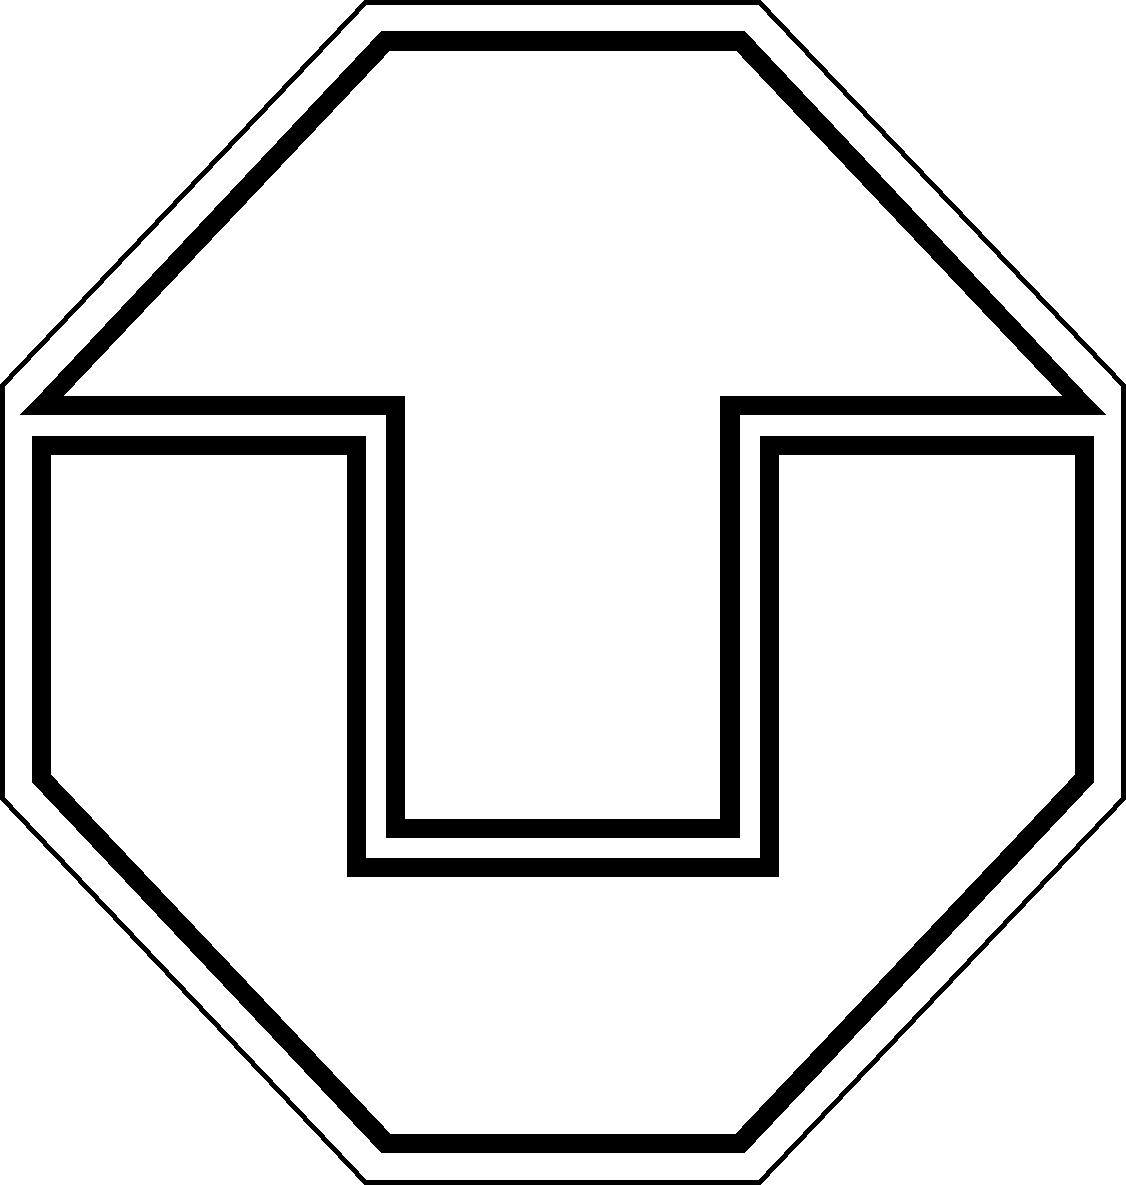
\includegraphics[width=3cm]{tu-logo}~\\[1cm]
\textsc{\LARGE Dresden University of Technology}\\[0.5cm]
\textsc{\Large Faculty of Computer Science}\\[0.2cm]
\textsc{\large Institute of Theoretical Computer Science}\\[0.2cm]
\textsc{\large Chair for Algebraic and Logical Foundations of Computer Science}\\[3cm]
\Huge Study's Thesis \\[1cm]
\huge Development and Analysis of Barrier Protocols\\[3cm]
\end{center}

\begin{flushleft} \large
	Author: Ronny Brendel \\
	Responsible university professor: Christel Baier \\
	Supervisors: Sascha Kl\"uppelholz \& Marcus V\"olp
\end{flushleft}

\vfill
\begin{flushright}
	\large October 2013
\end{flushright}

\end{titlepage}

\pagebreak
\newpage \thispagestyle{empty} \mbox{}
\pagebreak

%%%%%%%%%%%%%%%%%%%%%%%%%%%%%%%%%%%%%%%%%%%%%%%%%%%%%%%%%%%%%%%%%%%%%%%%%%%%%%%
%\section*{Aufgabenstellung}
%\label{sec:task}
%\begin{enumerate}
%	\item Literaturrecherche und ausf\"uhrlicher \"Uberblick aktuell genutzter Barrierenprotokolle sowie grunds\"atzlicher Implementierungsm\"oglichkeiten f\"ur Barrieren.
%	\item Untersuchung und Weiterentwicklung der von Nicolas Mc~Guire vorgeschlagenen Barriere.
%	\item Identifikation und Formalisierung der zentralen funktionalen Eigenschaften im Bezug auf Korrektheit sowie der quantitativen Eigenschaften zur Ermittlung der Performance von Barrierenprotokollen bez\"uglich Energieverbrauch und Geschwindigkeit.
%		\item Modellierung und Quantitative Analyse:
%			\begin{itemize}
%				\item Modellierung a) eines prominenten Vertreters von Barrierenprotokollen mit verteiltem Speicher, b) eines prominenten Vertreters von Barrierenprotokollen mit geteilten Speicher, c) des auf Mc~Guire beruhenden Barriereprotokolls jeweils im probabilistischem Model Checker PRISM.
%				\item Analyse und Vergleich der drei oben genannten Modelle im Bezug auf die in 3. identifizierten funktionalen sowie quantitativen Eigenschaften in PRISM. Wenn m\"oglich: Erg\"anzung des Performance-Vergleichs der drei Barrieren mittels messbasierter Methoden.
%			\end{itemize}
%		\item Zusammenfassung und Ausblick: Diskussion der in 4. gewonnenen Erkenntnisse
%\end{enumerate}
%
\section*{Task}
\label{sec:task}
\begin{enumerate}
	\item Literature research and detailed survey of currently used barrier protocols as well as implementation possibilities for barriers.
	\item Analysis and improvement of Nicolas Mc~Guire's proposed barrier.
	\item Identification and formalisation of key functional properties concerning correctness as well as quantitative aspects for determining performance of barrier protocols with regard to energy consumption and speed.
		\item Modelling and quantitative analysis:
			\begin{itemize}
				\item Modelling a) a prominent representative of barrier protocols for distributed memory, b) a prominent representative of barrier protocols for shared memory, c) the barrier protocol based on Mc~Guire's idea in each case using the probabilistic model checker PRISM.
				\item Analysis and comparison of the three above-mentioned models, regarding the functional as well as quantitative properties identified in 3., using PRISM. If possible: complement the performance evaluation of the three barriers using measurement-based methods.
			\end{itemize}
		\item Summary and outlook: Discussion of the insights gained in 4.
\end{itemize}

\pagebreak
\newpage \thispagestyle{empty} \mbox{}
\pagebreak

%%%%%%%%%%%%%%%%%%%%%%%%%%%%%%%%%%%%%%%%%%%%%%%%%%%%%%%%%%%%%%%%%%%%%%%%%%%%%%%
%\section*{Selbstst\"andigkeitserkl\"arung}
%\label{sec:integrity}
%Ich erkl\"are hiermit, dass ich die vorliegende Arbeit selbst\"andig und ohne Benutzung anderer als der angegebenen Hilfsmittel angefertigt habe. Die aus fremden Quellen w\"ortlich oder sinngem\"a\ss ~\"ubernommenen Gedanken sind als solche kenntlich gemacht. Ich erkl\"are ferner, dass ich die vorliegende Arbeit an keiner anderen Stelle als Pr\"ufungsarbeit eingereicht habe oder einreichen werde.

\section*{Statement of academic integrity}
\label{sec:integrity}
I hereby declare that I prepared this thesis independently and without use of tools other than specified. Foreign thoughts, taken literally or in spirit, are marked as such. I also declare that I have not filed the present work at any other location or will submit it.

\pagebreak
\newpage \thispagestyle{empty} \mbox{}
\pagebreak

%%%%%%%%%%%%%%%%%%%%%%%%%%%%%%%%%%%%%%%%%%%%%%%%%%%%%%%%%%%%%%%%%%%%%%%%%%%%%%%
\begin{abstract}
\todo
\begin{itemize}
	\item "don't use references in abstracts" - gernot's style guide
\end{itemize}

\end{abstract}
\pagebreak
\newpage \thispagestyle{empty} \mbox{}
\pagebreak

%%%%%%%%%%%%%%%%%%%%%%%%%%%%%%%%%%%%%%%%%%%%%%%%%%%%%%%%%%%%%%%%%%%%%%%%%%%%%%%
\renewcommand{\contentsname}{Table of contents}
\tableofcontents

\pagebreak
\newpage \thispagestyle{empty} \mbox{}
\pagebreak

%%%%%%%%%%%%%%%%%%%%%%%%%%%%%%%%%%%%%%%%%%%%%%%%%%%%%%%%%%%%%%%%%%%%%%%%%%%%%%%
\pagenumbering{arabic}
\section{Don't forget}
\begin{itemize}
	\item "don't overuse passive voice"
	\item explain use of 'thread' and 'process'. Probably in Section~\ref{ssec:existing-means}, when explaining the distinction between shared and distributed memory.
	\item be very aware where you use thread and process, and make sure the reader understands when the distinction does not matter
	\item make clear what is meant in the listings
		\begin{itemize}
			\item C-esque pseudo-code
			\item threadCount/processCount,  threadIndex/processIndex
			\item the code in the figures is executed on each thread. Each thread has an identifier between 0 and threadCount-1
			\item \& bit-wise \texttt{AND}, $|$ bit-wise \texttt{OR}, $\sim$ bit-wise \texttt{NOT}
			\item \texttt{x[$*$] := y} is short for assigning y to each element in x
			\item ?more?
		\end{itemize}
	\item mention that we assume atomic read and write at 32/64 bits a piece, when it matters
	\item explain cores vs processes, threads - we always assume threads, processes $>$= cores. Why. Find an appropriate spot to talk about this. I have marked a good spot in the text in Section~\ref{sssec:existing-currently-used-shared}
	\item "be forthright about the limitations and assumptions of your design. Also, make sure you justify any shortcuts/limitations convincingly"
	\item \texttt{me} vs \texttt{threadIndex} / \texttt{processIndex}, make its use coherent
	\item color use in diagrams should be consistent (same bars should have same color across multiple diagrams)
\end{itemize}

%%%%%%%%%%%%%%%%%%%%%%%%%%%%%%%%%%%%%%%%%%%%%%%%%%%%%%%%%%%%%%%%%%%%%%%%%%%%%%%
\section{Introduction}
\label{sec:introduction}
\begin{itemize}
	\item \todo watch out that the intention/laying down a continuous thread is strong enough ((1)barriers can be improved, (2)through pW/CS, (3)model checking is useful)
	\item what is a barrier
	\item usage example for barriers
	\item barriers are common in parallel programming. OpenMP's\cite{openmp} implicit barriers. MPI barriers (Rolf Rabenseifner\cite{rab00}). Relate to normal send/recv, because absolute numbers without relation are not helpful.
		\begin{itemize}
			\item HLRS, year 2000
			\item many calls,
			\item 5.3\% of all time spent inside MPI calls, 0.7\% of all CPU time, estimated 1.6\% of the barrier execution time is actual synchronization, 100\% minus 1.6\% is waiting for other processes to arrive, because of unbalanced computation, average 1852 micro seconds per call. (Figure~13 in paper)
			\item e.g. receive 12.9\% of all time spent inside MPI calls, 1.8\% of all cpu time, 33\% of the recv executation time is actual latency plus transfer time, 100\% minus 33\% is waiting for other processes to arrive, because of unbalanced comoputation, average 498 micro seconds per call.
		\end{itemize}
	\item motivation for researching barriers: Apply ideas of pW/CS\cite{pwcs} to other synchronization primitives, e.g. barriers in order to gain performance, where performance can be any important measure e.g. speed, energy efficiency, (say something about possible improvements that can still be made).
	\item summarize pW/CS
		\begin{itemize}
			\item usually concurrent programs work in a deterministic fashion. That is the order and partners of remote synchronization (locally, programs are obviously mostly deterministic) are predetermined. The algorithm is executed in a very controlled fashion. Same holds for synchronization primitives themselves. Faulty behavior is avoided at great cost.
			\item don't avoid inconsistency at all cost. Make errors detectable, or ignorable.
			\item use the inherent randomness\cite{mcg09}, induced by caching, scheduling, randomness (ECC, flash access e.g.) at hardware level (jitter), or short: complexity of today's computer systems, in order to view concurrent accesses as really random. Thus we are able to apply probabilistic algorithms and analyse these algorithms using tools of probability theory.
			\item design algorithms that have sufficiently high probability of success and tolerate faulty behaviour.
			\item build them so that on average, or in their intended use case, they perform better than their deterministic counterparts, where better might e.g. be faster, more energy efficient, resource preserving.
			\item data on the success is still rare, but it seems to be promising approach
			\item barriers can be improved. One possible way is through pW/CS.
		\end{itemize}
	\item how do we gather data on these algorithms to build confidence that they work properly, i.e. satisfy certain properties? And get a feeling for how they perform?
	\item Testing/Measurement (explain wording. Be aware of possible confusion) and model checking complement one another:
		\begin{itemize}
			\item Measurement is usually deterministic. If so, certain interesting states in a protocol are impossible to reach because of the randomness inherent to today's computers (add a short example? A special very case of a low level lock being contented?)
			\item Assuming you have randomized measurements, the probability to reach certain states in the protocol is so low that they are not revealed.
			\item Some parts of algorithms are performed in such a short time or need very exact preparation that it is practically impossible to analyse these parts using measurement. In this case model checking can be applied because it offers this granularity.
			\item Modelling has of course its own short comings. For example the state explosion problem.
			\item we can gain better quantitative insights into synchronization protocols by combining both measurement and model checking.
		\end{itemize}
	\item briefly explain the report structure
		\begin{itemize}
			\item existing stuff
				\begin{itemize}
					\item means to implement barriers
					\item currently used barriers
					\item idea to split barriers into orthogonal parts and think about them separately
				\end{itemize}
			\item new barriers
			\item analysis and comparison of one old for shared memory and one old for distributed memory against the new barriers
			\item conclusion \& future work
		\end{itemize}
\end{itemize}

%%%%%%%%%%%%%%%%%%%%%%%%%%%%%%%%%%%%%%%%%%%%%%%%%%%%%%%%%%%%%%%%%%%%%%%%%%%%%%%
\section{Background}
\label{sec:existing}

%%%%%%%%%%%%%%%%%%%%%%%%%%%%%%%%%%%%%%%
\subsection{Means to implement barrier protocols}
\label{ssec:existing-means}
\begin{itemize}
	\item \todo still feels like there should be some kind of wrap up or continuous thread :(
	\item evaluate what tools / APIs we have at our disposal to realize barrier protocols
	\item distinction between shared and distribute memory:
	\item threads vs processes. Explain use of these two words here.
	\item shared memory: all threads share one global memory. They are thus able to communicate by just writing to and reading from main memory.
	\item distributed memory: each process has its own private memory. Computation can only be done on private memory. Communication is explicitly done via an interconnect.
	\item programming these two memory architectures is very different, thus subsequently we will differentiate between these two worlds.
\end{itemize}

%%%%%%%%%%%%%%%%%%%%
\subsubsection{Shared memory}
\label{sssec:existing-means-shared}
\begin{itemize}
	\item normal load/store.
	\item atomic ops. An atomic operation is done in one instant without being interrupted by other memory accesses. E.g. add-fetch, compare-swap (is as old as 1970. No citations found. And perhaps not necessary). Never faster than normal read/write. (don't elaborate too much since we want a very high level view of the tools at our disposal)
	\item weaken consistency model. Consistency models describe restrictions on the order of visibility of memory accesses between multiple threads. In a thread, locally, the order is always the one specified by the program -- sequential. The default on x86 and most restrictive consistency model is sequential consistency. It is defined as follows:
		\begin{quote}
			The result of any execution is the same as if the operations of all the processors were executed in some sequential order, and the operations of each individual processor appear in this sequence in the order specified by its program. -- Lamport~\cite{sequentialconsistency}
		\end{quote}
		The most prominent weaker memory consistency model is release consistency~\cite{gha90}. Memory accesses appear unordered except so called \emph{release} and \emph{acquire} operations. No memory access that has been issued after an acquire operation is permitted to finish before this acquire operation. No memory access is allowed to finish later than the next release operation. Acquire and release encapsulate the memory accesses in between. Add a figure to explain. Generally speaking, weakening the consistency model gives improved performance, but one must pay attention while implementing concurrent programs, since the globally visible order of memory accesses will be different from the order specified by the source code. Improved performance: less waiting/queuing=more speed of operations, less need for wiring these restrictions in hardware.
	\item hardware support for barriers rare. Only found example: SGI UV 2000 systems\cite{sgiuv2000}
\end{itemize}

%%%%%%%%%%%%%%%%%%%%
\subsubsection{Distributed memory}
\label{sssec:existing-means-distributed}
\begin{itemize}
	\item categories
		\begin{itemize}
			\item synchronous message passing
				\begin{itemize}
					\item high level explanation (wikipedia?)
					\item relatively large overhead. Queueing. Waiting.
					\item all communicating partners need to be present at the same time and shake hands.
				\end{itemize}
			\item asynchronous message passing
				\begin{itemize}
					\item high level explanation (wikipedia?)
					\item similar overhead as synchronous message passing. not necessarily waiting.
					\item but partners still need to shake hands for information transfer.
				\end{itemize}
			\item remote memory access (RMA)
				\begin{itemize}
					\item accessing remote memory through read, write, (atomic operations), without the remote peer being actively involved.
					\item needs hardware support.
					\item less management overhead, better latency and throughput than message passing. Less buffering. Ideally no buffering - so called Zero-copy operations.
					\item distinction between coherent and non-coherent
					\item (a) coherent - remotely updated memory will be visible to the remote end eventually
					\item (b) non-coherent - no guarantee about visibility of remotely updated memory - needs active asking for changes by the remote end.
				\end{itemize}
			\item hardware support here is usual business e.g. Earth Simulator\cite{earthsimulator}, IBM Blue Gene/L\cite{bluegenel}, IBM Blue Gene/Q\cite{bluegeneq}, low-cost custom\cite{hoefler2006b}
			\item lossy communication e.g.
				\begin{itemize}
					\item most of today's synchronization protocols are based on a reliable communication layer e.g. TCP, InfiniBand's~\cite{infiniband} reliable connections. Unreliable communication is often supported though, e.g. UDP~\cite{udp}, InfiniBand's unreliable connections.
					\item Synchronization protocols for lossy channels could gain performance by performing less checks, like receive acknowledgements.
				\end{itemize}
		\end{itemize}
	\label{why-only-mpi}
	\item we specifically look at MPI\cite{mpi}. Why only MPI:
		\begin{itemize}
			\item standardized
			\item low-level
			\item portable, dist and shared mem, MPP, clusters of workstations, and combinations, independent of particular platform features or quantitative differences like latency/bandwidth
			\item very general and customizable. Supports many modes of operation.
			\item many implementations of the standard for many programming languages exist
			\item widely adopted in cluster computing / HPC, scientific computing.~\cite{mpiadoptiona, mpiadoptionb, mpiadoptionc}
		\end{itemize}
	\item only scratch surface of MPI, because:
		\begin{itemize}
			\item lots of details, because the standard is geared towards generality (supporting many different hardware platforms) and optimizability
			\item complicated semantics
			\item many of the details make no difference in protocol design/analysis
		\end{itemize}
	\item Don't use any MPI specific names. Keep it high-level
	\item MPI has synchronous message passing
		\begin{itemize}
			\item describe what you can do. How it is used.
			\item chapter 3.2 in \cite{mpi3}
			\item MPI\_Ssend, MPI\_Rsend (returns if no receiver is present), MPI\_Recv
		\end{itemize}
	\item MPI has asynchronous message passing
		\begin{itemize}
			\item describe what you can do. How it is used.
			\item chapter 3.7 in \cite{mpi3}
			\item MPI\_Isend, MPI\_Irecv
			\item MPI\_Wait, MPI\_Test
			\item MPI\_Cancel
			\item sync and async message passing can be mixed e.g. MPI\_Isend with a matching MPI\_Recv
		\end{itemize}
	\item MPI has asynchronous collectives
		\begin{itemize}
			\item chapter 5.12 in \cite{mpi3}
			\item explain shortly what this is about. You need to explain what collectives are.
			\item non-blocking collectives are not interesting as a building block for new barriers, because everyone has to take part and no cancellation of anything is possible.
		\end{itemize}
	\item MPI has RMA
		\begin{itemize}
			\item chapter 11 in \cite{mpi3}
			\item major changes from MPI 2.2\cite{mpi2} to 3.0\cite{mpi3onesided}
			\item we only consider MPI 3.0, because: More features. Subsumes MPI 2.2. It is already one year old. It is not yet realized by openmpi, but it is for mpich 3.0 and derivatives such as MVAPICH2\cite{mvapich}, Cray MPT\cite{craympt}
			\item MPI\_Win\_Create creates a so called 'window' of remotely shared memory among the participating processes. A process group is associated with a window.
			\item customizable attributes of windows: give the implementation guarantees about not using certain operations, not using certain operations at the same time, lowering memory consistency requirements for certain operations(accumulate).
			\item MPI\_WIN\_MODEL: explain SEPARATE and UNIFIED. One cannot set the MPI\_WIN\_MODEL to MPI\_WIN\_SEPARATE and MPI\_WIN\_UNIFIED myself. You can only ask for it. It has been proposed for MPI 3.1 to include being able to set a minimum necessary level. Algorithms for separate work on unified as well, but not necessarily the other way round.
			\item mpich 3.0.4 does MPI\_WIN\_UNIFIED.
			\item explaining epochs:
				\begin{itemize}
					\item an epoch is a period between two window synchronization calls
					\item rma calls data transfer calls like put, get, accumulate can only be used inside an epoch
					\item used to accumulate multiple calls etc -$\>$ efficiency
					\item MPI distinguishes access and exposure epochs, but we ignore these.
				\end{itemize}
			\item window sync
				\begin{itemize}
					\item active vs passive target communication (\cite{mpi3} page 437~)
					\item MPI\_Win\_Fence. Active target communication. Is a collective over all window group members. All outstanding RMA requests between group members will be finished. Implies a barrier.
					\item MPI\_Win\_Start, MPI\_Win\_Complete, MPI\_Win\_Post, and MPI\_Win\_Wait: active target communication. Similar to fence, but allows to specify the sync partners, and distinguishes between "command-issuing" and "remotely-accessed" processes.
					\item MPI\_WIN\_LOCK, MPI\_WIN\_UNLOCK: Passive target communication. No explicit participation of remote end in synchronization
					\item MPI\_Flush*: Passive target communication. Completes outstanding RMA calls, issued by the caller, at origin and a specifiable target before returning (or only at the origin).
					\item MPI\_Sync: Passive target communication. Used to synchronize the public and private part of the window in the separated model.
				\end{itemize}
			\item window sync assertions: NoPrecede, NoSucceed, NoStore, NoPut -$\>$ optimization
			\item MPI\_Put, MPI\_Get - unordered inside an epoch
			\item MPI\_Accumulate, MPI\_FetchAndOp, MPI\_CompareAndSwap influenced by specified memory order requirements. default is sequential consistency.
			\item list cases of undefined(implementation specific) behaviour: chapter 11.3 and 11.7 in \cite{mpi3}
				\begin{itemize}
					\item Buffers used in a MPI\_Put call should not be written to until the operation completes
					\item Buffers used in a MPI\_Get call should not be accessed until the operation completes
					\item The outcome of remote memory accesses to the same location is undefined. Except of course accumulate.
					\item concurrent local load/stores and RMA updates to the same location are undefined
					\item the outcome of a single process issuing multiple puts to the same location within an access epoch is undefined
					\item State that this makes it very hard to implement less restrictive synchronization primitives because the semantic requirements are already very strong in MPI. Lots of perhaps useless synchronization. Rather than undefined say: any order. Or at least make guarantee for the smallest units that are atomically committed to memory like primitive data types.
					\item perhaps state that in the following we will not implement, nor measure the performance of distributed memory algorithms. We will only measure shared memory stuff. But the will of course model check all the things.
				\end{itemize}
		\end{itemize}
\end{itemize}

\begin{itemize}
	\item most shared memory barriers rely on atomic operations
	\item most distributed memory barriers use synchronous message passing. These protocols have been implemented using RMA to improve efficeny, but they still behave exactly as if it was synchronous communication.
	\item as we will see in the next section
\end{itemize}

%%%%%%%%%%%%%%%%%%%%%%%%%%%%%%%%%%%%%%%
\subsection{Currently used barrier protocols}
\label{ssec:existing-currently-used}

%%%%%%%%%%%%%%%%%%%%
\subsubsection{Shared memory systems}
\label{sssec:existing-currently-used-shared}
\begin{itemize}
	\item explain short why only research in glibc and gnu openmp\cite{openmp}. closed source intel, microsoft, portland pgi, pathscale. pthreads und openmp open source und weit verbreitet. ?llvm?
	\item gnu openmp\cite{gomp}
		\begin{itemize}
			\item gcc 4.8.0, linux
			% gnu-openmp/gcc-4.8.0/libgomp/libgomp.h
			% gnu-openmp/gcc-4.8.0/libgomp/barrier.c
			% gnu-openmp/gcc-4.8.0/libgomp/config/linux/
			% gnu-openmp/gcc-4.8.0/libgomp/config/linux/bar.h
			% gnu-openmp/gcc-4.8.0/libgomp/config/linux/bar.c
			% gnu-openmp/gcc-4.8.0/libgomp/config/linux/futex.h (cpu_relax)
			% gnu-openmp/gcc-4.8.0/libgomp/config/linux/wait.h
			\item central counter barrier with atomic add and fetch
			\item Figure~\ref{fig:central-counter-no-reset}
				\begin{figure}[htbp]
					\centering
					\begin{minipage}
\centering
\begin{lstlisting}[mathescape, linewidth=10.4cm]
shared variables: integer barrier := threadCount
$\listingrule{10.4cm}$

atomic{barrier := barrier - 1}

wait until barrier = 0
\end{lstlisting}
\end{minipage}

					\caption{Pseudo code of the central counter barrier}
					\label{fig:central-counter-no-reset}
				\end{figure}
			\item explain algorithm in detail here
			\item is in reality more complex. For example back-off via a spin-counter $\sim$ 3ms. architecture specific. futexes\cite{franke2002}. kernel based mutexes. wait queues. sleeping. lowers spincount if core count $<$ thread count.
			\item talk about us assuming core count $>$= thread count. (from don't forget)
			\item reset built in. Last one to enter resets the barrier.
		\end{itemize}
	\item glibc's\cite{glibc} new pthreads library
		\begin{itemize}
			\item version 2.17. is in my ubuntu raring 13.04.
			% glibc/nptl/sysdeps/pthread/pthread.h
			% glibc/nptl/pthread_barrier_*
			% glibc/nptl/sysdeps/unix/sysv/linux/internaltypes.h
			\item central counter with locking instead of atomic add-fetch
			\item back-off through futexes (without spinning before)
			\item reset handled automatically (upon leaving the barrier every thread increments (atomically) the barrier by 1 so that it is max in the end)
		\end{itemize}
\end{itemize}

%%%%%%%%%%%%%%%%%%%%
\subsubsection{Distributed memory systems}
\label{sssec:existing-currently-used-distributed}
\begin{itemize}
	\item only MPI implementations. Why has already been explained in Section~\ref{why-only-mpi}.
	\item only openmpi and mpich. Explain why. (opensource. mpich is base of many others (name them). weit verbreitete implementationen.)
	\item openmpi
		\begin{itemize}
			\item version 1.7. not yet released.
			% ompi/mca/coll/tuned/coll_tuned_barrier.c :
			% ompi_coll_tuned_barrier_intra_recursivedoubling,
			% ompi_coll_tuned_barrier_intra_bruck
			% ompi/mca/coll/tuned/coll_tuned_decision_fixed.c
			\item $n \neq 2^k \rightarrow$ dissemination\cite{hensgen1988} using sync sendrecv
			\item $n = 2^k \rightarrow$ recursive doubling (explanation e.g. in \cite{hoefler2005})
			\item back-off hard to determine. probably through OPAL\_THREAD\_(UN)LOCK in the end
			\item resetting (in both algorithms) not necessary since sendrecv sets up itself newly everytime.
			\item architecture specific for infiband. e.g. dissemination using RMA \cite{hoefler2006a}
			\item Figure~\ref{fig:dissemination-no-reset}
			\item state that we use an RMA representation of the algorithm. Maybe state why. Writing is sending. Reading is Receiving so to speak.
				\begin{figure}[htbp]
					\centering
					\begin{lstlisting}[mathescape]
shared variables: boolean
                  barrier[processCount][processCount]
local variables:  integer dist
initialization:   barrier[*][*] := false

for dist := 1; dist < numThreads; dist := dist $\times$ 2 {
	to   := (processIndex + dist) (mod processCount)
	from := (processIndex - dist) (mod processCount)
	
	barrier[to][processIndex] := true
	
	wait until barrier[processIndex][from] = true
}
\end{lstlisting}


					\caption{Pseudo code of the dissemination barrier}
					\label{fig:dissemination-no-reset}
				\end{figure}
			\item explain algorithm in detail here
			\item things to explain
				\begin{itemize}
					\item each array (first index) is located on the respective process's memory
				\end{itemize}

		\end{itemize}
	\item mpich
		\begin{itemize}
			\item many mpi implementations are based on mpich (e.g. mvapich2, intel mpi, cray mpi,
			\item many can not be inspected because source is closed
			\item version 3.0.4. current today
			% src/mpi/coll/barrier.c : MPIR_Barrier_intra
			\item log2 Dissemination with sendrecv. same as openmpi
		\end{itemize}
	\item dissemination can also be used for shared memory\cite{hoefler2013}
\end{itemize}

%%%%%%%%%%%%%%%%%%%%%%%%%%%%%%%%%%%%%%%
\subsection{Barrier building blocks}
\label{ssec:building-blocks}
\begin{itemize}
	\item latency/computation trade-off
	\item resetting:
		\begin{itemize}
			\item how is resetting handled in currently used barriers?
			\item switching between barriers using a variable (as in the nmg/ronny barrier - 'left' variable)
			\item use 3 barriers reset barrier x+2 when you finished barrier x. switch between the barriers by checking if barrier x+2 is reset or not (as in central-counter-with-reset). Describe in pseudo code as well, maybe.
			\item if variable space permits it you can also change the variables to 'counters' and modify all checks to ask for numbers modulo round + a check that you are in the proper round
		\end{itemize}
	\item back-off
	\item thread count $<$= cores, thread count $>$ cores
	\item combining: we can combine barrier protocols. Explain how. Reap benefits, mitigate shortcomings. Adapt to topology (explain. Node shared mem, internode dist mem., different interconnect topologies) aware.
\end{itemize}

%%%%%%%%%%%%%%%%%%%%%%%%%%%%%%%%%%%%%%%%%%%%%%%%%%%%%%%%%%%%%%%%%%%%%%%%%%%%%%%
\section{Three new barriers}
\label{sec:new}
\begin{itemize}
	\item put some introductory text here
	\item \todo pay attention where to draw the line between this section and the analysis in the next section (perhaps, leave some/most of the analysis for the next section)
	\item \todo elegantly transition to Ronny's fancy barrier (distributed memory case). Suddenly talking about processes and remote/local memory is bad.
\end{itemize}
%%%%%%%%%%%%%%%%%%%%%%%%%%%%%%%%%%%%%%%
\subsection{Mc Guire/Ronny}
\label{ssec:new-nmg}
\begin{itemize}
	\item original idea by Nicholas Mc Guire was given to me in a private communique.
	\item modification of the original protocol resulted in Figure~\ref{fig:nmg-ronny-with-reset}
	\item first appearance in bre13\cite{bre13}. Slight modification since then "remembers others" considered here. Don't explain in detail what the modification is and does, since the reader has no knowledge of the previous version and I don't want to explain all of it.
		\begin{figure}[htbp]
			\centering
			\begin{minipage}
\centering
\begin{lstlisting}[mathescape, linewidth=12.1cm]
constants:        meBit:=$2^{threadIndex}$, full:=$\sum_{i=0}^{threadCount-1}2^i$
shared variables: integer entry := 0, integer exit := 0,
                  boolean left := false
local variables:  integer copy
$\listingrule{12.1cm}$

if left = false {

	do {
		copy := (copy & $\sim$meBit) | entry
		if copy & meBit = 0 {
			copy  := copy | meBit
			entry := copy
		}
	} while copy $\neq$ full and left = false

	left := true
	exit := 0

} else if left = true {

	do {
		copy := (copy & $\sim$meBit) | exit
		if copy & meBit = 0 {
			copy := copy | meBit
			exit := copy
		}
	} while copy $\neq$ full and left = true

	left  := false
	entry := 0
}
\end{lstlisting}
\end{minipage}

			\caption{Pseudo code of Mc Guire/Ronny's barrier}
			\label{fig:nmg-ronny-with-reset}
		\end{figure}
	\item high-level explanation
	\item detailed walk through one iteration
	\item advantage: no atomic ops
	\item resetting is integrated. Needs a little less space than the approaches shown in Section~\ref{ssec:building-blocks}
	\item Limited to 64 threads in this version. But one can modify the protocol to use an array of bit masks, representing a big bit mask. Updating the bit mask will then only be done on the element where the updating thread is itself located on. This way we only write one 64 bit value which is committed atomically. If we would attempt to write more than one element, we would run into consistency problems. Reading the shared variable will then read the whole array instead.
\end{itemize}

%%%%%%%%%%%%%%%%%%%%%%%%%%%%%%%%%%%%%%%
\subsection{Ronny's simple barrier}
\label{ssec:new-simple}
\begin{itemize}
	\item new and shiny. Read mostly, write exactly once. In contrast to Mc Guire/Ronny's barrier.
	\item How did I come up with the idea?
	\item Figure~\ref{fig:ronny-simple-no-reset}
		\begin{figure}[htbp]
			\centering
			\documentclass[class=article, border=10pt]{standalone}

\usepackage[latin1]{inputenc}
\usepackage{tikz}
\usetikzlibrary{shapes,arrows,positioning}
\begin{document}
\pagestyle{empty}

%styles
\tikzstyle{->}   = [draw, -latex']
\tikzstyle{o}    = [draw, circle]
\tikzstyle{box}  = [draw, rectangle, rounded corners]

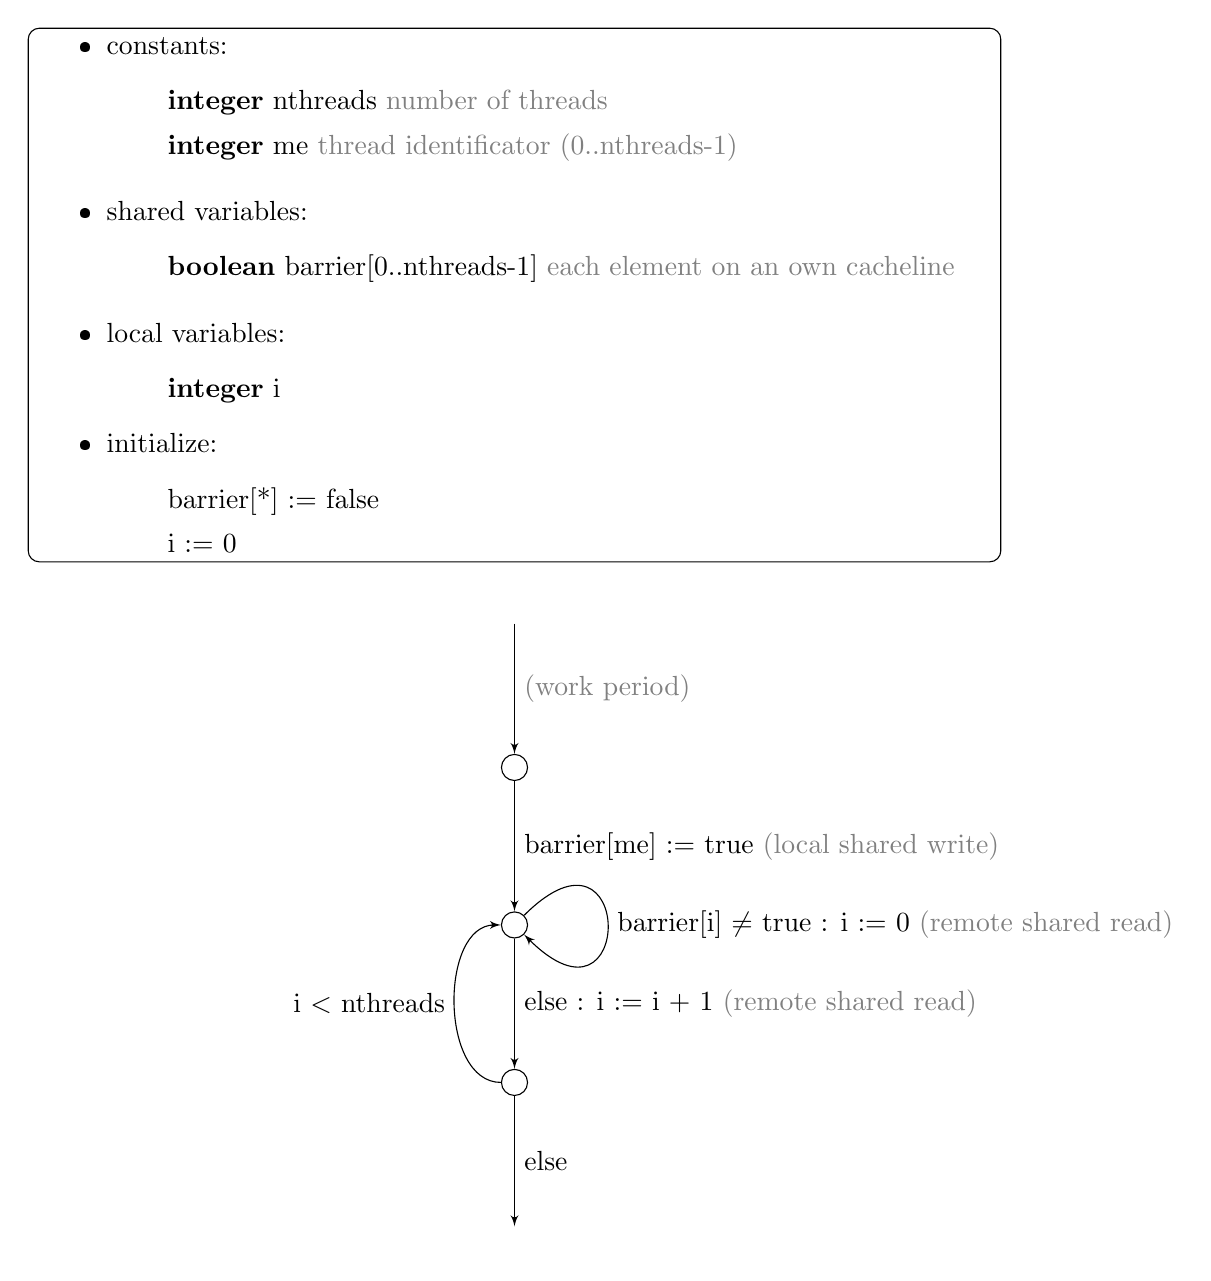
\begin{tikzpicture}[node distance = 2.0cm, auto]


% preamble
\node [box, align=left] (pre)  {
	\begin{minipage}{12cm}
		\begin{itemize}
			\item constants:
				\begin{itemize}
					\item[] \textbf{integer} nthreads {\color{gray} number of threads}
					\item[] \textbf{integer} me \color{gray} thread identificator (0..nthreads-1)
				\end{itemize}
			\item shared variables:
				\begin{itemize}
					\item[] \textbf{boolean} barrier[0..nthreads-1] \color{gray}each element on an own cacheline
				\end{itemize}
			\item local variables:
				\begin{itemize}
					\item[] \textbf{integer} i
				\end{itemize}
			\item initialize:
				\begin{itemize}
					\item[] barrier[*] := false
					\item[] i := 0
				\end{itemize}
		\end{itemize}
	\end{minipage}
};

% nodes
\node [o, below of=pre, draw=none, yshift=-2cm]  (init) {};
\node [o, below of=init]                         (1)    {};
\node [o, below of=1]                            (2)    {};
\node [o, below of=2]                            (3)    {};
\node [o, below of=3, draw=none]                 (done) {};

%  edges
\path [->] (init) edge                                      node       {\color{gray}(work period)}                                (1);
\path [->] (1)    edge                                      node       {barrier[me] := true \color{gray}(local shared write)}     (2);
\path [->] (2)    edge [loop, distance=2cm, out=45, in=-45] node       {barrier[i] $\ne$ true : i := 0 \color{gray}(remote shared read)} (2);
\path [->] (2)    edge                                      node       {else : i := i + 1 \color{gray}(remote shared read)}       (3);
\path [->] (3)    edge [out=180, in=180]                    node[left] {i $<$ nthreads}                                           (2);
\path [->] (3)    edge                                      node       {else}                                                     (done);

\end{tikzpicture}

\end{document}



			\caption{Pseudo code of Ronny's simple barrier}
			\label{fig:ronny-simple-no-reset}
		\end{figure}
	\item explanation here.
	\item one array element per cache line to avoid false sharing\cite{falsesharing}
	\item every thread writes into the array element he owns. Indicated by his threadIndex.
	\item do not mention (analysis section instead): in contrast to the central-counter barrier the assignments to shared variables can be done in parallel, since the variables written are not the same, no are they on the same cache line.
	\item (do not mention. Is in the analysis) many read accesses, but since data is cached upon the first read the latency is only significant once per array element / cache line. i.e. when the thread arrives and writes his array element to be \texttt{true} and when a thread reads it after it has been written by it's owner.
	\item advantage: no atomic ops
	\item (do not mention. Is in the analysis) larger memory cost than central counter, Mc Guire/Ronny. They number of barriers per thread team should be 1 at most, thus the memory overhead is still negligible.
	\item The barrier is destructive in the sense that it cannot be executed multiple times in a row. One way to circumvent this is to modify the algorithm to use a repetition counter instead of a boolean (since we have one date per cache line we allocated the space anyways) and keep track of it. The algorithm would then atomically increase the counter instead of the assignment in line 4. We use a 64 bit integer variable for this. It will not overflow over so we don't need to consider this case (If you could run one barrier each clock cycle on a 3GHz machine you would need roughly 200 years to overflow it).
	\item another small improvement would be to keep track of the first couple of successfully read entries and skip those when repeating the loop. For simplicity's sake and modelling we will not consider this optimization.
\end{itemize}

%%%%%%%%%%%%%%%%%%%%%%%%%%%%%%%%%%%%%%%
\subsection{Ronny's fancy barrier}
\label{ssec:new-fancy}
\begin{itemize}
	\item variation of Ronny's simple barrier where not only will the own presence be stored, but the presence of other processes, we know have arrived, as well. Similar to the "remember others" modification of the Mc Guire/Ronny barrier.
	\item evaluation has shown that cache latency is so low, that the additional computation this mechanism introduces, makes this algorithm run slower on shared memory systems than the unmodified one. Thus we will now switch to a distributed memory scenario where communication latency is much higher. If we assume RMA for communication we can use the protocol without modification.
	\item Figure~\ref{fig:ronny-fancy-no-reset}
		\begin{figure}[htbp]
			\centering
			\begin{minipage}
\centering
\begin{lstlisting}[mathescape, linewidth=11.5cm]
constants:        me := processIndex, meBit := $2^{me}$,
                  full := $\sum_{i=0}^{\mathit{processCount}-1}2^i$
shared variables: integer barrier[processCount]
initialization:   barrier[*] := full
$\listingrule{11.5cm}$

barrier[me] := full & $\sim$meBit;

i := processIndex + 1 (mod processCount)
do {
	while barrier[me] & $2^i$ = 0 and i < processCount {
		i := i + 1
	}

	if i < processCount {
		barrier[me] := barrier[me] & barrier[i]
	} else {
		i := 0
	}
} while barrier[me] $\neq$ 0
\end{lstlisting}
\end{minipage}

			\caption{Pseudo code of Ronny's fancy barrier}
			\label{fig:ronny-fancy-no-reset}
		\end{figure}
	\item each array element is located in the memory of the respective process.
	\item Only the own element is written. Only remote reading.
	\item When a process reads remotely he is informed of other processes, the remote end knows, have arrived.
	\item probabilistic runtime. Depending on circumstances the protocol will finish in more or less steps (or perhaps successful non-zero reads). It is not predetermined what is communicated and with whom.
	\item We will quantify this effect in Section~\ref{sec:analysis}.
	\item advantage: no atomic ops. The writing does not have to be atomic, since processes only write to local memory, and no inconsistent data can be read since 64 bit reads and writes are atomic.
	\item more computational overhead (bit shuffling) for less communication.
	\item discuss resetting through triple barrier. Perhaps, briefly hint that this kind of resetting can be added to any barrier (perhaps add a listing how this would look like (the spin model should have it, or one of the pseudo code files)), more on this in the section on the orthogonal design of barriers.
	\item restricted to 64 threads. An extension to arrays of bit masks, similar to the Mc Guire/Ronny barrier, should not pose a problem.
\end{itemize}

%%%%%%%%%%%%%%%%%%%%%%%%%%%%%%%%%%%%%%%%%%%%%%%%%%%%%%%%%%%%%%%%%%%%%%%%%%%%%%%
\section{Analysis and comparison}
\label{sec:analysis}
\begin{itemize}
	\item \todo maybe distinguish extreme cases vs more normal cases. And the spectrum in between -- adds structure -- is nice.
	\item In this section we will evaluate one commonly used barrier for each shared memory and distributed memory architectures and pit them against one novel protocol in each category.
	\item Early evaluations have shown the Mc Guire/Ronny's barrier to perform worse than the central counter barrier, whereas Ronny's simple barrier shows promise. Therefore we restrict our attention to the latter.
	\item For the shared memory case the central counter barrier (Figure~\ref{fig:central-counter-no-reset} in Section~\ref{sssec:existing-currently-used-shared}) is pitted against Ronny's simple barrier (Figure~\ref{fig:ronny-simple-no-reset} in Section~\ref{ssec:new-simple}).
	\item For distributed memory architectures the dissemination barrier (Figure~\ref{fig:dissemination-no-reset} in Section~\ref{sssec:existing-currently-used-distributed}) and Ronny's fancy barrier (Figure~\ref{fig:ronny-fancy-no-reset} in Section~\ref{ssec:new-fancy}) are compared. (explain choice with a few words? -- ref existing-currently-used?)
	\item we will not implement, nor measure the performance of both distributed memory protocols -- because Ronny's barrier cannot easily be implemented due to MPI restrictions explained in Section~\ref{sssec:existing-means-distributed}. But it is of course possible to implement such an algorithm using lower level APIs, for example the Mellanox InfiniBand-Verbs API~\cite{mellanox}. Doing so goes beyond the scope of this thesis.
	\item In our evaluations we always assume no back-off strategy is used. Each algorithm polls busily on the requested variable until the desired value is read. Threads do not wait sleeping or use callback mechanisms. The topic of back-off strategies is a large and intricate subject in its own right and goes beyond the scope of this thesis.
	\item We ignore the topic of resetting barriers as well, as introducing a resetting scheme alters the protocol only in a minuscule way. And the simplicity and reduced model size is much more appreciable than the benefit of addressing this minor concern in the analysis. -- we will come back to resetting again in Section~\ref{ssec:building-blocks}
	\item The analysis is split into three parts: general properties, measurement and model checking.
\end{itemize}

%%%%%%%%%%%%%%%%%%%%%%%%%%%%%%%%%%%%%%%
\subsection{General properties}
\label{ssec:analysis-general}
\begin{itemize}
	\item group properties into measurable and non-measurable (model checking, sharp looking at)
	\item present considerations of interest about the chosen algorithms.
\end{itemize}

%%%%%%%%%%%%%%%%%%%%
\subsubsection{Central counter vs Ronny's simple barrier}
\label{sssec:analysis-general-shared}
\begin{itemize}
	\item give an introduction to cache. Factor of 10-100 between cache and main memory access latency. Cache line invalidation and fetching make up most of the time used in such protocols. Thus it's important to look at these.
	\item PHASES: both algorithms are performed in two phases. A writing phase and a reading phase.
	\item In the writing phase of the central counter barrier concurrently issued add-fetch operations will be queued (because atomic ops on a single variable). On the other hand Ronny's simple barrier allocates one cache line per array element. Thus all writes to shared memory can be executed in parallel. If all threads arrive at the same instant, writing can be sped up to a factor of $\mathit{threadCount}$ in comparison to executing serialized write operations. In more balanced scenarios this effect diminishes.
	\item The reading phase of the central counter barrier reads a single variable repeatedly. The cache line this variable resides on will be invalidated for each core exactly $\mathit{threadCount} - 1$ times (disregarding outside influences) ((, thus each core fetches the variable at most $\mathit{threadCount} - 1$ times)).
	\item The reading phase of Ronny's simple barrier needs to read each array element once until it can make a decision whether to leave or repeat the loop. Each array element is invalidated exactly once. Thus each array element, from the viewpoint of one thread, has to be fetched from memory at most twice. From then on it is cached and quickly accessible.
	\item the central counter barrier has the obvious advantage in this phase. How big this advantage is depends heavily on the underlying hardware. For example if the cache line prefetcher predicts the access pattern of the reading phase of Ronny's simple barrier, those reads can be executed in parallel.
	\item The central counter barrier is quicker during busy waiting, whereas Ronny's simple barrier performs well during writing. We attempt to quantify this behaviour using benchmarks and model checking in the following subsections.
	\item MEMORY: the central counter barrier needs a logarithmic amount of memory in the number of threads (i.e. 64 bits, for up to $2^{64}$ threads), whereas Ronny's simple barrier needs a linear amount -- $\mathit{threadCount} \times 64$ bytes, assuming a cache line is 64 bytes. This looks like a lot, but since shared memory systems rarely exceed 512 cores, a maximum of only about 32KiB of memory would be used. 64 byte per thread. Furthermore one thread team needs only one barrier and repeat it. There would be no benefit in allocating the memory for more than one.
\end{itemize}

%%%%%%%%%%%%%%%%%%%%
\subsubsection{Dissemination vs Ronny's fancy barrier}
\label{sssec:analysis-general-distributed}
\begin{itemize}
	\item For the dissemination barrier the number of remote writes is exactly $n \times \lceil \log _2~n \rceil$ -- $n$ processes times $\lceil \log _2~n \rceil$ rounds. Dissemination remotely writes more than the minimum needed in order to gain speed over the straightforward gather + broadcast approach, which is $2 \times (n-1)$ writes in $2 \times  \lceil \log _2~n \rceil$ rounds. Add picture about the minimum. (a linear and a tree-esque).
	\item Reading is only done locally.

%  +--------+        +--------+             round (2)
%  v        |        v        |
%  0 <- 1   2 <- 3   4 <- 5   6 <- 7        round (1)
%  ^                 |
%  +-----------------+                      round (3)

	\item Ronny's fancy barrier needs between $2 \times (n-1)$ and $n \times (n-1)$ successful (non-zero) remote reads. Writing is only done locally.
	\item dissemination needs exactly $\lceil \log _2~n \rceil$ rounds. Ronny's fancy barrier does not have rounds and tries reading from the next process regardless of whether a remote read has been successful (non-zero) where the dissemination barrier waits for its designated communication partner.
	\item needing $\lceil \log _2~n \rceil$ rounds is obviously worse than $\log _2~n$. This especially means that from $\lfloor \log _2~n \rfloor$ to $\lfloor \log _2~n \rfloor + 1$ the number of rounds increases by 1. Therefore, for core counts other that are not a power of two, the performance degrades. Super wasteful shows a more balanced picture with increasing core counts where dissemination has jumps at power of two core counts. (elaborate? Since we do not benchmark and we probably won't model check larger numbers, we won't be able to quantify this). Benchmarks on shared memory have shown this to be true. (perhaps future work?: A way to mitigate this would be to reduce the number of processes executing the additional round to as few as possible and then do a normal power-of-2 dissemination barrier)
	\item MEMORY: The memory requirements of the dissemination barrier and Ronny's fancy barrier are the same. Each process uses some local memory to keep track of the other processes. The exact number depends on the implementation. In principle for both algorithms $\lceil \log _2~n \rceil$ bits per process suffice. The dissemination variant shown in Figure~\ref{fig:dissemination-no-reset} uses a total of $n \times n$ bits, but, since each thread communicates only with $\lceil \log _2~n \rceil$ other threads, a modified index calculation would allow it to work with $n \times \lceil \log _2 ~n \rceil$ bits. The memory usage is minuscule either way.
	\item talk about the progress problem when one process is missing.
		\begin{itemize}
			\item number of blocked processes doubles each round.
			\item each one of these blocked processes then needs to finish the still to do rounds until the protocol succeeds

% normal:
%  phase 1:  0 -> 1 -> 2 -> 3 -> 4 -> 5 -> 6 -> 7 -> 0
%  phase 2:  0 ------> 2 ------> 4 ------> 6 ------> 0
%                 1 ------> 3 ------> 5 ------> 7 ------> 1
%  phase 3:  0 ----------------> 4 ----------------> 0
%                 1 ----------------> 5 ----------------> 1
%                      2 ----------------> 6 ----------------> 2
%                           3 ----------------> 7 ----------------> 3
%
%  now suppose one process (e.g. 4) has not yet arrived
%
%  phase 1:  0 --> 1 ---> 2 ---> 3 --> (4) -x> 5 ---> 6 ---> 7 ---> 0
%  phase 2:  0 ---------> 2  --------> (4) -----x---> 6 ----------> 0
%                  1  ---------> 3 ---------> (5) ----x----> 7 --------> 1
%  phase 3:  0 ----------------------> (4) -----------x-----------> 0
%                 1 ------------------------> (5) -----------x----------> 1
%                        2 ------------------------> (6) ----------x----------> 2
%                               3 ------------------------> (7) ---------x---------> 3
%
%  who knows whom while process 4 is missing:
%   =round 1=           =round 2=           =round 3=           =the best possible outcome=
%   7 know themselves     + 4 new               + 0 new               maximum would be 49
%   + 6 new                                     total is 17
%   0: 0           7    0: 0         6 7    0: 0         6 7    0: 0 1 2 3   5 6 7
%   1: 0 1              1: 0 1         7    1: 0 1         7    1: 0 1 2 3   5 6 7
%   2:   1 2            2: 0 1 2            2: 0 1 2            2: 0 1 2 3   5 6 7
%   3:     2 3          3:   1 2 3          3:     2 3          3: 0 1 2 3   5 6 7
%   5:         5        5:         5        5:         5        5: 0 1 2 3   5 6 7
%   6:         5 6      6:         5 6      6:         5 6      6: 0 1 2 3   5 6 7
%   7:           6 7    7:           6 7    7:           6 7    7: 0 1 2 3   5 6 7
%
% maximum progress is ~2*n of a maximum of (n-1)*(n-1). (Perhaps find out the exact formulas)
%
% another advantage is that: when the last process arrives he will fetch all processes in one go
%
			\item non-power of 2 process counts: The number of blocked processes still doubles per round. The ratio of who is blocked in what round is thus worse than in the power of 2 case.
			\item quantification of these effects is done in the model checking chapter (both number of messages and the progress problem!). And mention here that you will do it. (if not beware of talking about it here!)
		\end{itemize}
\end{itemize}

%%%%%%%%%%%%%%%%%%%%%%%%%%%%%%%%%%%%%%%
\subsection{Model checking}
\label{ssec:analysis-modelchecking}
\begin{itemize}
	\item introduce layers. Program graphs (vs lower level) vs tools. -- adds structure -- might be nice
	\item SPIN\cite{spin, hol97}, PRISM\cite{prism, knp09}
\end{itemize}

%%%%%%%%%%%%%%%%%%%%
\subsubsection{Preliminaries}
\label{sssec:analysis-modelchecking-preliminaries}
\begin{itemize}
	\item \todo cut out what is not needed in the following sections (like time bounded eventually, or immediate rewards, etc)
	\item \todo maybe add transition rewards
	\item continuous-time Markov chains.
	\item further details in textbooks like \cite{kul95, ks76}
	\item if $S$ is a finite set, then a distribution on $S$ is a function $\nu:S \rightarrow [0,1]$ with $\sum\limits_{s \in S} \nu (s) = 1$. For $U \subseteq S$, $\nu (U)$ is a shortform notation for $\sum\limits_{s \in U} \nu (s)$.
	\item CTMC tuple $\mathcal{M} = (S, \mathit{Act}, R, \mu)$, where $S$ is a finite state space, $Act$ a finite set of action names and $R$ a function of type $S \times \mathit{Act} \times S \rightarrow \mathbb{R}_{\ge 0}$, called the rate matrix of $\mathcal{M}$. $\mu$ is a distribution on $S$ specifying the probabilities for the initial states.
	\item $s \xrightarrow{\lambda : \alpha} s'$ if $R(s, \alpha, s') = \lambda > 0$ means $\mathcal{M}$ has a transition from $s$ to $s'$ with action label $\alpha$ and rate $\lambda$
	\item $\lambda$ specifies the rate of the exponential distribution. That is the probability for the transition $s \xrightarrow{\lambda : \alpha} s'$ to be ready for firing some time in the interval $[0,t]$ is $1-e^{- \lambda t}$. The average delay  of this transition is $1 / \lambda$.
	\item If $R(s, \alpha, s') = 0$ then there is no transition in $\mathcal{M}$ from $s$ to $s'$ via $\alpha$.
	\item choice between enabled transition is made through the race condition. Thus, the time-abstract probability to fire a particular transition $s \xrightarrow{\lambda : \alpha} s'$ is $P(s, \alpha, s') = \lambda / E(s)$ where $E(s)$ is the exit rate of state $s$, i.e., the sum of the rates of all outgoing transitions of state $s$. The probability that $s \xrightarrow{\lambda : \alpha} s'$ will fire within $t$ time units is then $P(s, \alpha, s') \cdot (1 - e^{- E(S) \cdot t})$.
	\item paths in a CTMC are sequences of consecutive transitions augmented by the time points when they are taken.
	\item For the analysis of such transition systems we employ the logic CSL \cite{assb96, bhhk00, knp07}. (my formulation)
	\item To specify measurable sets of infinite paths, we will use an LTL-like notation, such as $\lozenge T$ ("eventually T") where $T \subseteq S$ denotes the set of all infinite paths that contain at least one $T$-State. $\lozenge^{\le t}$ is the time-bounded eventually with time bound $t$. Similarly, $\mathcal{U}$ denotes the until operator and $\mathcal{U}^{\le t}$ the time-bounded until with time bound $t$.
	\item Instead of naming states we will oftentimes use state predicates and propositional formulas to describe sets of states. Their meaning will be obvious from the context. (my formulation)
	\item we will also study reward based properties formalized using the logic CSRL \cite{bhhk00, knp07}
	\item This requires the extension of $\mathcal{M}$ by a reward function $\mathit{rew} : S \rightarrow \mathbb{R}_{\ge 0}$ where $\mathit{rew}$ specifies the reward to be earned per time  unit when staying in state $s$. For finite paths one can then reason about cumulative, reachability and instantaneous rewards.
	\item Suppose $\pi$ is a finite path where the underlying state sequence is $s_1 s_2 ...s_n$ and let $t_0 = 0$ and $t_i$ the time point where $\pi$ takes the $i$-th transition.
	\item The accumulated reward of $\pi$ is
		\begin{center}
			$\mathit{Rew}(\pi) = \mathlarger{\sum}\limits_{i=0}^{n-1} (t_{i+1} - t_i) \cdot \mathit{rew}(s_i)$
		\end{center}
		It is the sum, over all states but the last, of the state reward multiplied by the time spent in this state.
	\item cumulative reward
		\begin{center}
		$\mathrm{CumRew}(\pi, t) = \mathit{Rew}(s_0..s_j)$
		\end{center}
		where $j = min \{ i~|~t_i \ge t \}$
	\item reachability reward
		\begin{center}
			$\mathrm{ReaRew}(\pi, \Phi) = \mathit{Rew}(s_0..s_j)$
		\end{center}
		where $j = min \{ i~|~s_i \models \Phi \}$
	\item instantaneous reward
		\begin{center}
			$\mathrm{InsRew}(\pi , t) = \mathlarger{ \sum }\limits_{i=0}^{n}~\pi_i(t) \cdot rew(s_i)$
		\end{center}
		where $\pi_i(t)$ is the probability of being in state $s_i$ at time $t$
	\item the extension of these functions from paths to states and models is done the usual way and can be found in \cite{bhhk03}
	\item in the analysis of the protocols we will for example deal with the reward function that assigns value \texttt{base\_rate} (or 1) to each state. In this case $\mathrm{ReaRew}(T)$ can be interpreted as the average cycle count to reach $T$.
\end{itemize}

%%%%%%%%%%%%%%%%%%%%
\subsubsection{Modelling} %AE: modeling, BE: modelling
\label{sssec:analysis-modelchecking-modelling}
\begin{itemize}
	\item distinct models for functional and quantitative properties
	\item because resetting and repetition only needed for functional properties + we can save state space by stripping the model of unnecessary information for the quantitative analysis
	\item ordinary (non-stochastic) transition systems for functional models and CTMCs for quantitative models
	\item Spin\cite{spin, hol97} for model checking functional properties
	\item PRISM\cite{prism, knp09} for quantitative analysis
	\item in the following graphs we will use control flow diagrams and CTMCs
	\item The CTMCs of the protocols will be composed of multiple modules.
	\item synchronization between modules on the CTMC level is done via synchronizing actions.
	\item composed modules are executed interleaved except if transitions require synchronizing actions. A synchronizing action is an action that can be issued by at least two modules. A transition with such an action can only fire if all modules, that are able to fire this action eventually, are presently in a state where they can fire it. The rate of such a transition is determined by any one module. For each synchronization action, in our case, only one module will specify a rate for this action.
	\item This corresponds to the following SOS rules
	\item If no other module uses the action $\alpha$ \\
		\begin{center}
			$\mathlarger{\frac{s \xrightarrow{\lambda : \alpha} s'}{\langle s , \overline{x} \rangle \xrightarrow{\lambda : \alpha} \langle s', \overline{x} \rangle}}$}
		\end{center}
	\item $\overline{x}$ stands for the tuple of local state of all other modules
	\item if $\alpha$ is used by two modules \\
		\begin{center}
			$\mathlarger{\frac{s \xrightarrow{\lambda : \alpha} s', t \xrightarrow{\alpha} t'}{\langle s, t , \overline{x} \rangle \xrightarrow{\lambda : \alpha} \langle s', t', \overline{x} \rangle}}$
		\end{center}
	\item analogous rules can be stated for more than two modules sharing an action.
\end{itemize}

%%%%%%%%%%
\paragraph{Shared memory}
\label{sssec:analysis-modelchecking-modelling-shared-memory}
\begin{itemize}
	\item todo reason why modelling cache?
		\begin{itemize}
			\item memory access determines performance of synchronization protocols
			\item memory access is cached so that effectively we only deal with cache latency
		\end{itemize}
	\item shared memory variable encapsulated in own CTMC modules.
	\item We identify a variable with the cache line it resides on.
	\item each thread has one copy of such a cache line.
	\item synchronization between cache line copies and with other modules of a model, like the actual program to be modelled, is done via synchronizing actions. The triggering thread of a cache operation determines the rate of the operation.
	\item we use an MSI cache coherency protocol extended by support for atomic operations. MSI model is the most basic cache model and explanations on it can readily be found online\cite{msi}.
	\item A cache line copy can be in one of four states. \emph{modified}, means the thread has the only up-to-date copy of the cache line and all other copies are marked invalid. \emph{shared}, which means the core has an up-to-date copy, but zero or more other threads have a correct copy, too. \emph{invalid}, meaning the local copy is not up-to-date. We extend these three states by a fourth named \emph{atomic}. It is the same as modified, except that between $\mathit{atomic\_begin}$ and $\mathit{atomic\_end}$ the access to this variable is blocked. Figure~\ref{fig:shared-memory-control-flow} shows how a cache line copy changes its state depending on events occurring. The solid transitions are triggered by events occurring on the thread owning the cache line copy, whereas dashed transitions are due to events issued indirectly by actions of other threads.
	\item CTMC Figure~\ref{fig:shared-memory-control-flow}
		\begin{figure}[htbp]
			\centering
			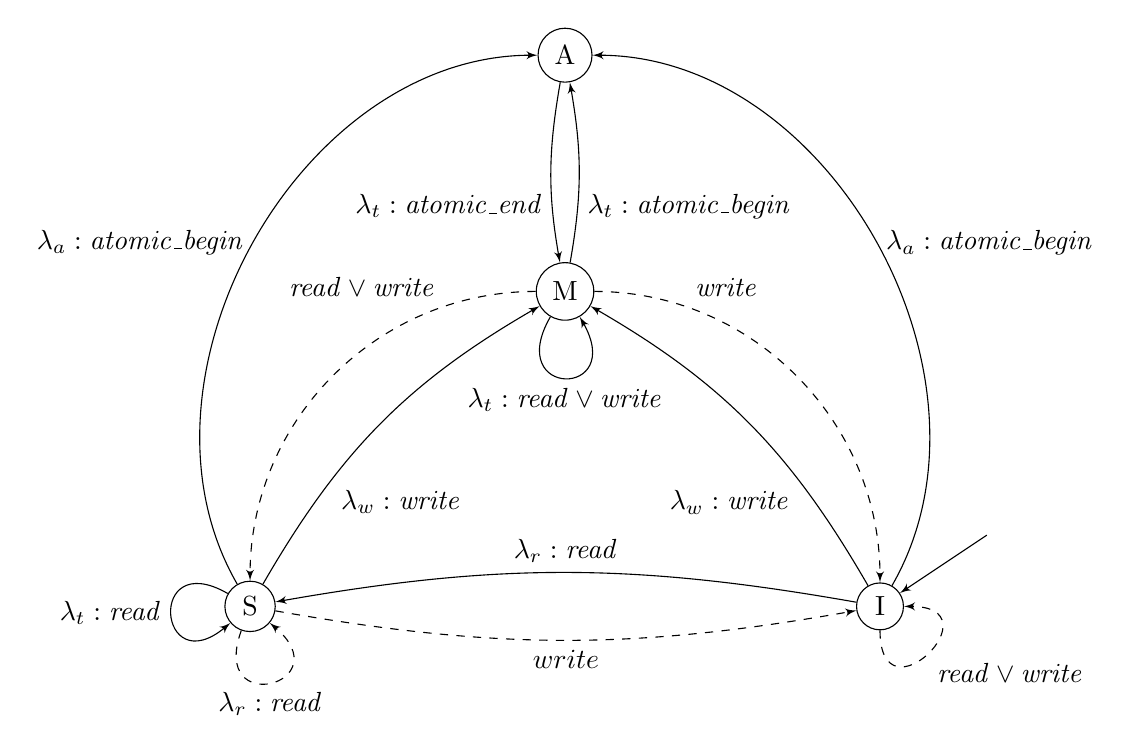
\begin{tikzpicture}[]

% nodes
\node [o]            at (  0  ,  3   ) (A)    {A};
\node [o]            at (  0  ,  0   ) (M)    {M};
\node [o]            at ( -4.0, -4.0 ) (S)    {S};
\node [o]            at (  4.0, -4.0 ) (I)    {I};
\node [o, draw=none] at (  5.5, -3.0 ) (init) {};

%  edges
\path [->]
  (init) edge                                                 node []                     {}                                     (I)

  (A)    edge [in=100, out=260]                               node [left, pos=0.7]        {$\lambda_t : \mathit{atomic\_end}$}   (M)

  (M)    edge [in=-80, out=80]                                node [right, pos=0.3]       {$\lambda_t: \mathit{atomic\_begin}$}  (A)
  (M)    edge [loop, distance=1.2cm, in=-60, out=240]         node [below] {$\lambda_t: \mathit{read} \lor \mathit{write}$}      (M)
  (M)    edge [dashed, in=90, out=180]                        node [above left, pos=0.2]  {$\mathit{read} \lor \mathit{write}$}  (S)
  (M)    edge [dashed, in=90, out=0]                          node [above right, pos=0.2] {$\mathit{write}$}                     (I)

  (S)    edge [in=180, out=120]                               node [left]                 {$\lambda_a : \mathit{atomic\_begin}$} (A)
  (S)    edge [in=210, out=60]                                node [below right, pos=0.3] {$\lambda_w : \mathit{write}$}         (M)
  (S)    edge [loop, distance=1.2cm, in=220, out=150]         node [left]                 {$\lambda_t : \mathit{read}$}          (S)
  (S)    edge [loop, dashed, distance=1.2cm, in=320, out=250] node [below]                {$\lambda_r : \mathit{read}$}          (S)
  (S)    edge [dashed, in=190, out=-10]                       node [below]                {$write$}                              (I)

  (I)    edge [in=0, out=60]                                  node [right]                {$\lambda_a : \mathit{atomic\_begin}$} (A)
  (I)    edge [in=-30, out=120]                               node [below left, pos=0.3]  {$\lambda_w : \mathit{write}$}         (M)
  (I)    edge [in=10, out=170]                                node [above]                {$\lambda_r : \mathit{read}$}          (S)
  (I)    edge [loop, dashed, distance=1.2cm, in=0, out=-90]   node [below right]          {$\mathit{read} \lor \mathit{write}$}  (I);

\end{tikzpicture}

			\caption{CTMC of a shared memory variable}
			\label{fig:shared-memory-control-flow}
		\end{figure}
	\item For example if a core reads a variable, it first needs to make sure that all other cores take notice and change its cache line copy state to shared in case it was modified before. After this the core fetches the cache line, marks its copy shared and continues reading the variable.
	\item taken from complex-lab, rephrase: The timings of shared read and shared write are as follows. A read on a modified or shared variable does not imply any extra work. It can immediately use the cached data. Therefore we consider this operation instantaneous. If a read is done on an invalid copy, it has to first fetch an up-to-date copy of the cache line and make sure all other cores are notified before it can proceed. This usually takes around 50 CPU cycles. A write on a modified variable is instantaneous, since all other cores do not have an up-to-date copy and therefore do not have to be notified. If the cache line in question is in a shared or invalid state, we first have to wait until all other cores follow the request to invalidate their copies of the cache line. After this we can safely mark our copy modified and write to it. This operation usually takes around 100 cycles.
	\item taken from complex-lab, rephrase: The number of cycles these operations take is strongly dependent on the CPU itself. For the CTMC model we assume a cache read to use 50 cycles and a cache write to use 100 cycles. The rates of the transitions corresponding to the described events is then the reciprocal of the cycle time: 1, $\frac{1}{50}$ or $\frac{1}{100}$.
	\item $\lambda_c$, $\lambda_r$, $\lambda_w$, $\lambda_a$ one cycle, read, write, atomic\_begin rate. Reciprocal of the average number of cycles needed for each of these actions
	\item explain CTMC behaviour and work around through setting atomic\_begin to something higher than write, although normally it would be just that
	\item explain to move atomic rate to atomic end to make parallel and serial code look different (explain how parallel and serial doesn't make a difference for interleaved CTMCs)
\end{itemize}

%%%%%%%%%%
\paragraph{Central counter barrier}
\label{sssec:analysis-modelchecking-modelling-central-counter}
\begin{itemize}
	\item repeat variables and initial configuration from the algorithm box
	\item Algorithm explained in Section~\ref{sssec:existing-currently-used-shared}
	\item Control flow diagram Figure~\ref{fig:central-counter-control-flow}
		\begin{figure}[htbp]
			\centering
			\begin{minipage}
\centering
\begin{lstlisting}[mathescape, linewidth=10.4cm]
shared variables: integer barrier := threadCount
$\listingrule{10.4cm}$

atomic{barrier := barrier - 1}

wait until barrier = 0
\end{lstlisting}
\end{minipage}

			\caption{Control flow diagram of the central counter barrier}
			\label{fig:central-counter-control-flow}
		\end{figure}
	\item rates for reading writing and atomic operations are determined by the module for the shared variable \texttt{barrier}
	\item the synchronization to the shared variable module is hinted at in grey
	\item The control flow has been augmented by one rate that the resulting CTMC will use. $\lambda_{work}$ is the work rate, meaning the time spent doing actual work. It is used to add an initial distribution to the model so that we can control how the arrival times of the threads at the barrier are distributed. In particular not all threads arrive at the exact same instant in time at the barrier, which is an extreme case.
	\item atomic op consists of multiple smaller transitions: begin atomic (locks the variable), read barrier, decrement it, write barrier, end atomic (releases the lock).
	\item functional model does resetting and repetition. Three barriers, as described in~\ref{ssec:building-blocks}. (if you did not describe it there, you have to do it here)
\end{itemize}

%%%%%%%%%%
\paragraph{Ronny's simple barrier}
\label{ssssec:analysis-modelchecking-modelling-ronny-simple}
\begin{itemize}
	\item repeat variables and initial configuration from the algorithm box
	\item Algorithm explained in Section~\ref{ssec:new-simple}
	\item Control flow diagram Figure~\ref{fig:ronny-simple-control-flow}
		\begin{figure}[htbp]
			\centering
			\documentclass[class=article, border=10pt]{standalone}

\usepackage[latin1]{inputenc}
\usepackage{tikz}
\usetikzlibrary{shapes,arrows,positioning}
\begin{document}
\pagestyle{empty}

%styles
\tikzstyle{->}   = [draw, -latex']
\tikzstyle{o}    = [draw, circle]
\tikzstyle{box}  = [draw, rectangle, rounded corners]

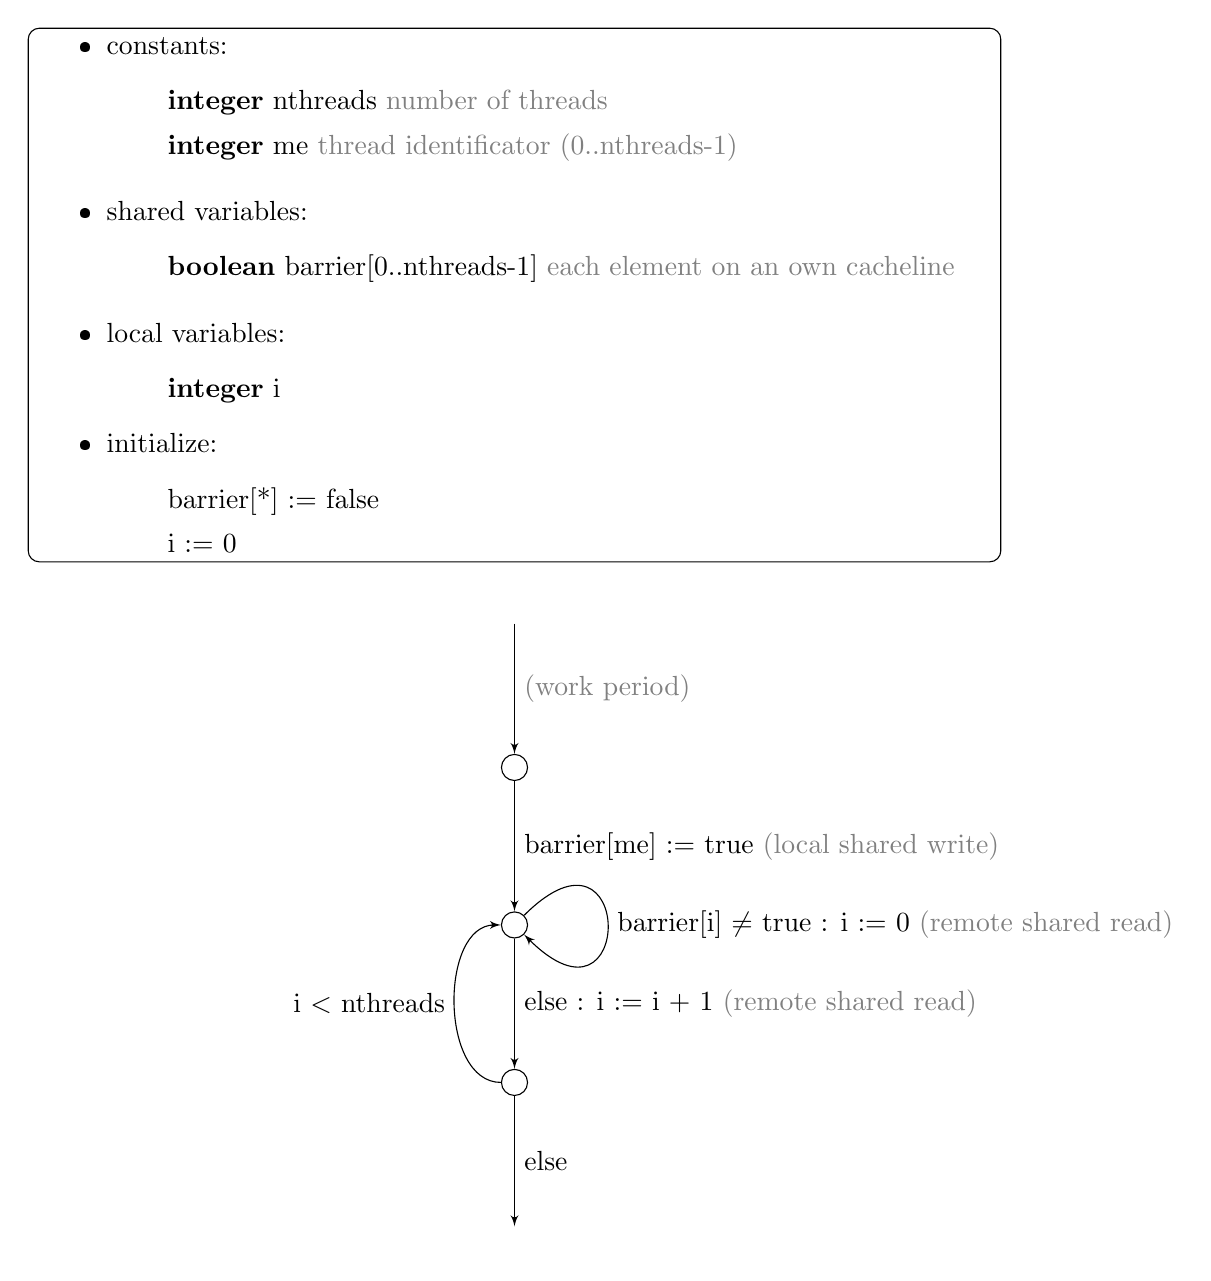
\begin{tikzpicture}[node distance = 2.0cm, auto]


% preamble
\node [box, align=left] (pre)  {
	\begin{minipage}{12cm}
		\begin{itemize}
			\item constants:
				\begin{itemize}
					\item[] \textbf{integer} nthreads {\color{gray} number of threads}
					\item[] \textbf{integer} me \color{gray} thread identificator (0..nthreads-1)
				\end{itemize}
			\item shared variables:
				\begin{itemize}
					\item[] \textbf{boolean} barrier[0..nthreads-1] \color{gray}each element on an own cacheline
				\end{itemize}
			\item local variables:
				\begin{itemize}
					\item[] \textbf{integer} i
				\end{itemize}
			\item initialize:
				\begin{itemize}
					\item[] barrier[*] := false
					\item[] i := 0
				\end{itemize}
		\end{itemize}
	\end{minipage}
};

% nodes
\node [o, below of=pre, draw=none, yshift=-2cm]  (init) {};
\node [o, below of=init]                         (1)    {};
\node [o, below of=1]                            (2)    {};
\node [o, below of=2]                            (3)    {};
\node [o, below of=3, draw=none]                 (done) {};

%  edges
\path [->] (init) edge                                      node       {\color{gray}(work period)}                                (1);
\path [->] (1)    edge                                      node       {barrier[me] := true \color{gray}(local shared write)}     (2);
\path [->] (2)    edge [loop, distance=2cm, out=45, in=-45] node       {barrier[i] $\ne$ true : i := 0 \color{gray}(remote shared read)} (2);
\path [->] (2)    edge                                      node       {else : i := i + 1 \color{gray}(remote shared read)}       (3);
\path [->] (3)    edge [out=180, in=180]                    node[left] {i $<$ nthreads}                                           (2);
\path [->] (3)    edge                                      node       {else}                                                     (done);

\end{tikzpicture}

\end{document}



			\caption{Control flow diagram of ronny's simple barrier}
			\label{fig:ronny-simple-control-flow}
		\end{figure}
	\item each element of the array \texttt{barrier} is located in an own cache line. Therefore each thread has \texttt{threadCount} cache line copy modules, one for each element in the array. In total a CTMC model of this protocol has $\mathtt{threadCount}^2$ cache line copy modules plus $\mathtt{threadCount}$ thread modules.
	\item As described in the previous paragraph, $\lambda_{work}$ is the work rate and all other rates are determined by the cache line copy modules.
	\item functional model does resetting and repetition using a counter instead of bools as described in Section~\ref{ssec:building-blocks} (if you did not describe it there, you have to do it here)
	\item functional model splits some of the transitions to allow for more interleaving, thus more errors can be revealed.
\end{itemize}

%%%%%%%%%%
\paragraph{Dissemination barrier}
\label{ssssec:analysis-modelchecking-modelling-dissemination}
\begin{itemize}
	\item repeat variables and initial configuration from the algorithm box
	\item no special module for distributed memory, since all variables are independently stored in the local memory of each process. There is no influence that copies data between processes other then the user-specified program itself.
	\item Algorithm explained in Section~\ref{sssec:existing-currently-used-distributed}
	\item Control flow diagram augmented with rates: Figure~\ref{fig:dissemination-control-flow}
		\begin{figure}[htbp]
			\centering
			\begin{lstlisting}[mathescape]
shared variables: boolean
                  barrier[processCount][processCount]
local variables:  integer dist
initialization:   barrier[*][*] := false

for dist := 1; dist < numThreads; dist := dist $\times$ 2 {
	to   := (processIndex + dist) (mod processCount)
	from := (processIndex - dist) (mod processCount)
	
	barrier[to][processIndex] := true
	
	wait until barrier[processIndex][from] = true
}
\end{lstlisting}


			\caption{Augmented Control flow diagram of the dissemination barrier}
			\label{fig:dissemination-control-flow}
		\end{figure}
	\item As in the two previous paragraphs $\lambda_{work}$ is the work rate.
	\item we assume all local operations to be much quicker, ten to a thousand times, than remote operations. Therefore we assign the rate $\lambda_c$ (one CPU cycle) to local operations. $\lambda_p$, which is assigned to remote write (put) operations, is assigned a rate of $\frac{1}{100}$. This value is, like the shared memory rates, hardware-dependent. For simplicity's sake we assume a remote transfer to take 100 cycles.
	\item one could make this more fine grained by introducing separate rates for local reading and writing.
	\item \texttt{to} and \texttt{from} are shorthands for \texttt{processIndex $\pm$ dist (mod processCount)}
	\item In the CTMC model, resulting from unwinding this control flow diagram, a put onto a remote process is represented as a synchronized action, so the target process stores the new value in its CTMC module.
	\item functional model does resetting and repetition with a counter instead of bools as described in Section~\ref{ssec:building-blocks}.
\end{itemize}

%%%%%%%%%%
\paragraph{Ronny fancy barrier}
\label{ssssec:analysis-modelchecking-modelling-ronny-fancy}
\begin{itemize}
	\item repeat variables and initial configuration from the algorithm box
	\item Algorithm explained in Section~\ref{ssec:new-fancy}
	\item Control flow diagram augmented with rates: Figure~\ref{fig:ronny-fancy-control-flow}
		\begin{figure}[htbp]
			\centering
			\begin{minipage}
\centering
\begin{lstlisting}[mathescape, linewidth=11.5cm]
constants:        me := processIndex, meBit := $2^{me}$,
                  full := $\sum_{i=0}^{\mathit{processCount}-1}2^i$
shared variables: integer barrier[processCount]
initialization:   barrier[*] := full
$\listingrule{11.5cm}$

barrier[me] := full & $\sim$meBit;

i := processIndex + 1 (mod processCount)
do {
	while barrier[me] & $2^i$ = 0 and i < processCount {
		i := i + 1
	}

	if i < processCount {
		barrier[me] := barrier[me] & barrier[i]
	} else {
		i := 0
	}
} while barrier[me] $\neq$ 0
\end{lstlisting}
\end{minipage}

			\caption{Augmented Control flow diagram of ronny's fancy barrier}
			\label{fig:ronny-fancy-control-flow}
		\end{figure}
	\item Rates are like in previous section, except we now use remote read (get) with a rate of $\lambda_g = \frac{1}{100}$.
	\item functional model does resetting and repetition using three barriers as described in~\ref{ssec:building-blocks}.
\end{itemize}

%%%%%%%%%%%%%%%%%%%%
\subsubsection{Functional properties}
\label{sssec:analysis-modelchecking-functional-properties}
\begin{itemize}
	\item intro text here
	\item in this section we will use \emph{thread} and \emph{process} interchangeable, because for the modelling side the wording makes no difference.
	\item LTL as logic, Spin as model checker
	\item $T$ is the set of all threads
	\item $left_t$ is a predicate describing all states where thread $t$ has passed the barrier
	\item $entered_t$ is a predicate describing all states where thread $t$ has passed the initial work period
	\item \textbf{A:} \emph{a thread may only exit the barrier if all threads have entered it}
		\begin{center}
			$\square \big( ~ ( \exists t \in T . \mathit{left_t} ) \implies \forall s \in T. \mathit{entered_s} ~ \big)$
		\end{center}
	\item \textbf{B:} \emph{if all threads entered the barrier, they will all leave it in a finite amount of time}
		\begin{center}
			$\square \big( ~(\forall t \in T . \mathit{entered_t} ) \implies \forall s \in T. \lozenge \mathit{left_s} ~ \big)$
		\end{center}
	\item A and B are the only two properties a barrier protocol must satisfy
	\item A could be seen as safety and B as liveness of the protocol
	\item yes it works.
\end{itemize}

%%%%%%%%%%%%%%%%%%%%
\subsubsection{Quantitative properties}
\label{sssec:analysis-modelchecking-quantitative-properties}
\begin{itemize}
	\item intro text here
	\item in this section we will use \emph{thread} and \emph{process} interchangeable, because for the modelling side the wording makes no difference. (same is in section before)
	\item CSRL as logic, PRISM as model checker
\end{itemize}

%%%%%%%%%%
\paragraph{Identification and formalisation}
\label{ssssec:analysis-modelchecking-quantitative-properties-identification}
\begin{itemize}
	\item which parameters to variate
		\begin{itemize}
			\item thread count. Maximum 4 is considered. Model checking limitations bla.
			\item work rate. Variate the distribution of the times the threads enter the barrier.
		\end{itemize}
	\item interesting points in time
		\begin{itemize}
			\item (A) first thread entered the barrier
			\item (B) last thread entered the barrier
			\item (C) first thread left the barrier
			\item (D) last thread left the barrier
			\item (E) (only for central counter and ronny's simple) the last thread finished writing
		\end{itemize}
	\item resulting properties
		\begin{itemize}
			\item $T$ is the set of all threads
			\item \textbf{A:} \emph{Average time until the first thread enters the barrier}
				\begin{center}
					$\mathrm{ReaRew}(\exists t \in T . \mathit{entered_t} )$
				\end{center}
			\item \textbf{B:} \emph{Average time until the last thread enters the barrier}
				\begin{center}
					$\mathrm{ReaRew}(\forall t \in T . \mathit{entered_t} )$
				\end{center}
			\item \textbf{C:} \emph{Average time until the first thread leaves the barrier}
				\begin{center}
					$\mathrm{ReaRew}(\exists t \in T . \mathit{left_t} )$
				\end{center}
			\item \textbf{D:} \emph{Average time until the last thread leaves the barrier}
				\begin{center}
					$\mathrm{ReaRew}(\forall t \in T . \mathit{left_t} )$
				\end{center}
			\item \textbf{E:} \emph{Average time until the last thread finished writing}
				\begin{center}
					$\mathrm{ReaRew}(\forall t \in T . \mathit{done\_writing_t} )$
				\end{center}
			\item and combinations of these to get measures like (D-B) last in until last out.
		\end{itemize}
	\item \todo additional properties of dissemination and ronny's fancy
		\begin{itemize}
			\item rounds. one is in round x, but not yet one in the next. all are at least in round x, but not yet all are in the next.
			\item number of remote transfers. \todo needs transition rewards.
			\item progress. Number of processes known to have arrived for each process. $\frac{0.. n*(n-1)}{n*(n-1)}$
		\end{itemize}
\end{itemize}

%%%%%%%%%%
\paragraph{Results}
	\begin{itemize}
		\item technical modification of queries to yield cycle counts instead of raw time.
		\item central counter vs ronny's simple
			\begin{itemize}
				\item work = 100. Very Small.
				\item last to last, last to first Figure~\ref{fig:cs-work-100-B-C-D}
					\begin{figure}[htbp]
						\centering
						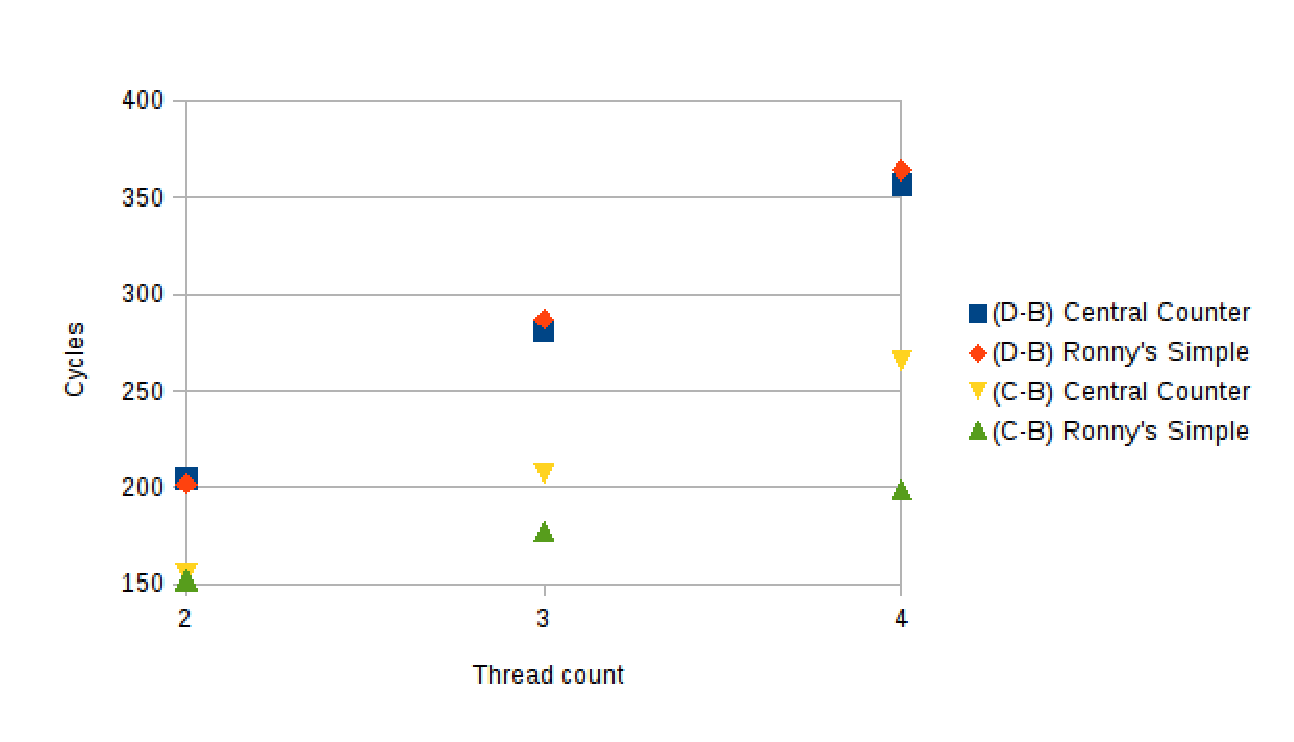
\includegraphics[width=8cm]{charts/cs-work-100-B-C-D}
						\caption{Expected running time of the shared memory barriers}
						\label{fig:cs-work-100-B-C-D}
					\end{figure}
					\begin{itemize}
						\item similarly fast when considering the last one to finish
						\item ronny's simple faster for the first one to leave
					\end{itemize}
				\item distribution of total time spent: Figure~\ref{fig:cs-work-100-partition}
					\begin{figure}[htbp]
						\centering
						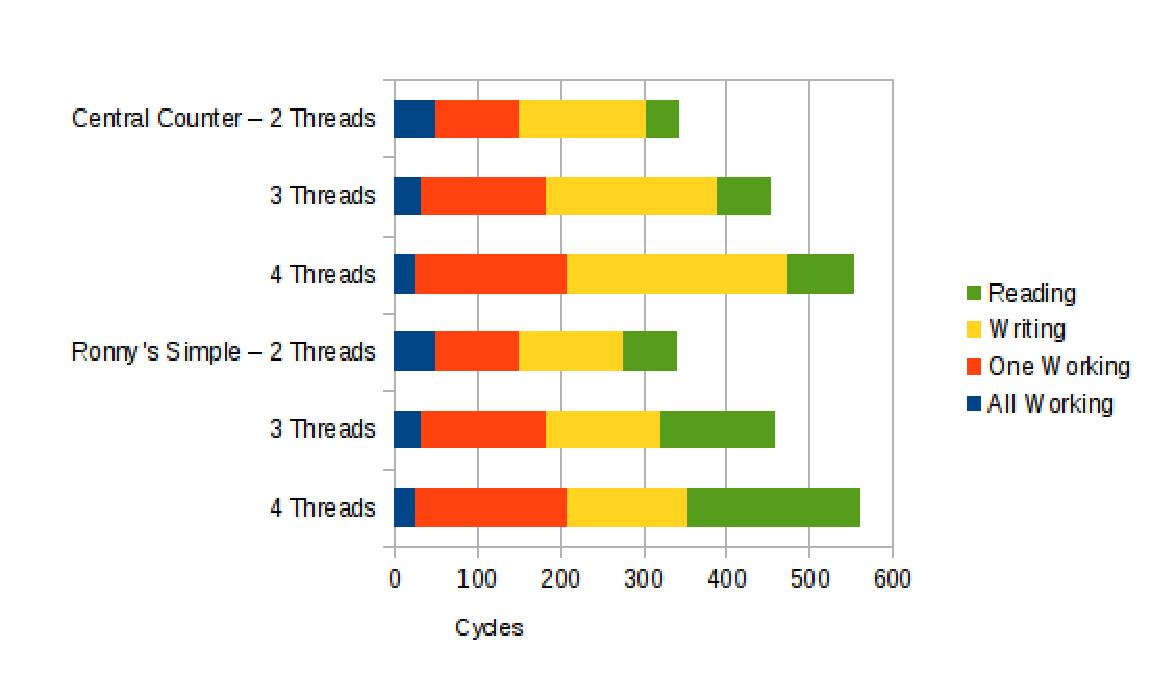
\includegraphics[width=8cm]{charts/cs-work-100-partition}
						\caption{Distribution of total time spent}
						\label{fig:cs-work-100-partition}
					\end{figure}
					\begin{itemize}
						\item stacked fashion. Writing starts during one working. Reading starts during writing.
						\item work is equal for everyone, obviously
						\item first thread leaves a few cycles after writing is done. Because the last one to write its value will
							read the completed barrier and immediately leaves.
						\item last thread exits when reading is done. Because when reading is done, we are done.
						\item writing, as expected, takes longer for central counter and reading takes longer for ronny's simple
						\item all parts take longer as well, since CTMC semantic makes interleaved transitions get an exit rate of $\lambda / n$ for n modules each with rate $\lambda$, so that the expected time of a parallel execution is $\sum_{i=1}^{n} \frac{1}{i \cdot \lambda}}$  time rather than $1 / \lambda$ for $n$ interleaved modules / concurrent threads. Especially reading for central counter (2: 50, 3:75, 4:92 cycles). Normally this period is expected to be nearly the same for all thread counts.
					\end{itemize}
				\item reading vs writing: Figure~\ref{fig:cs-work-100-percent}
					\begin{figure}[htbp]
						\centering
						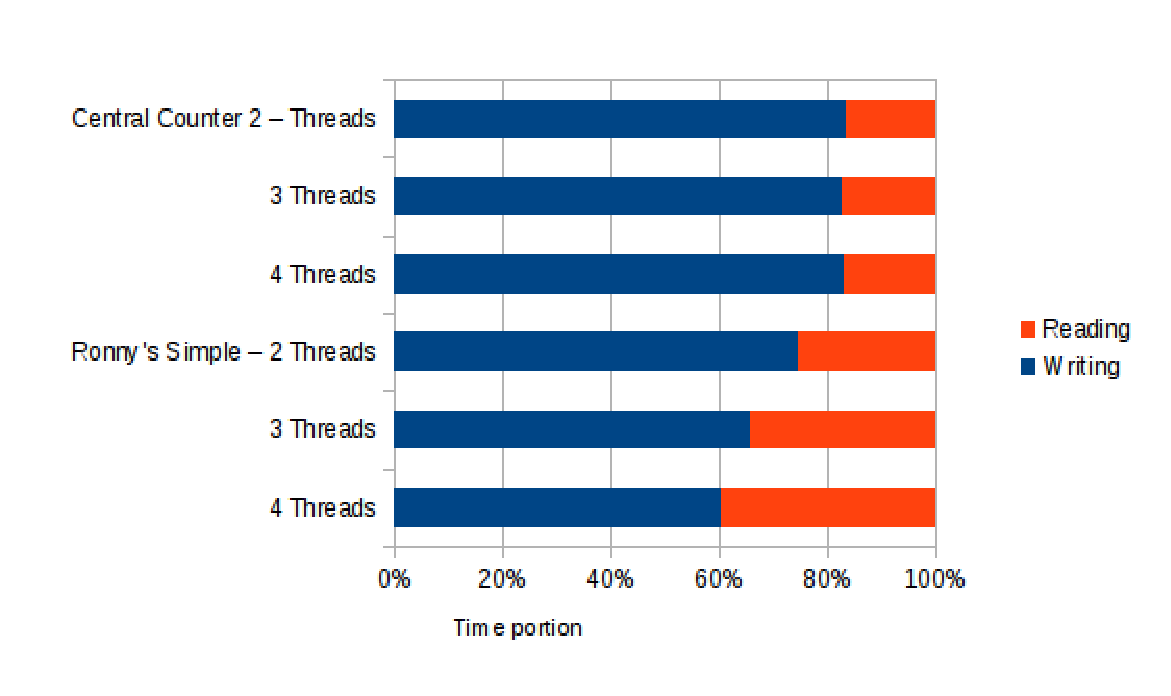
\includegraphics[width=8cm]{charts/cs-work-100-percent}
						\caption{Percentage of time spent writing vs time spent reading}
						\label{fig:cs-work-100-percent}
					\end{figure}
					\begin{itemize}
						\item another picture showing writing vs reading.
						\item atomic ops queue up. Parallel writes do not.
						\item writing for ronny's simple is expected to take less time than shown here (100 across the board instead of 2:125, 3:138, 4:146), for the same reason as reading takes longer as expected for the central counter barrier.
					\end{itemize}
				\item work=1000. Still very small.
				\item last to last, last to first Figure~\ref{fig:cs-work-1000-B-C-D}
					\begin{figure}[htbp]
						\centering
						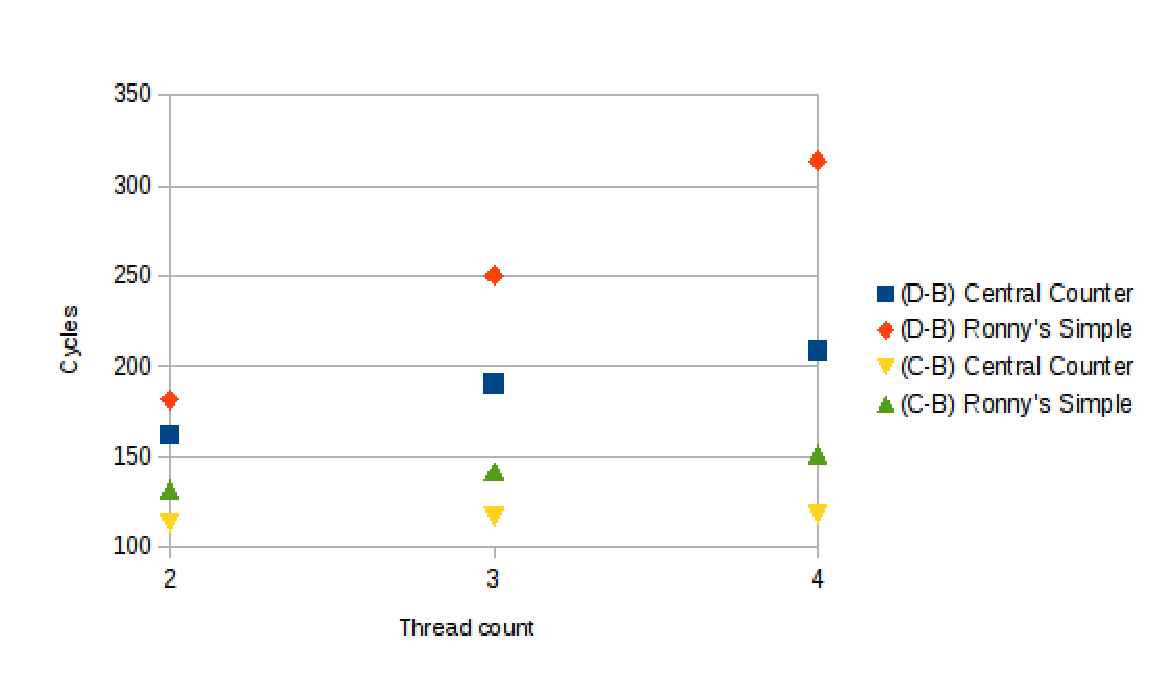
\includegraphics[width=8cm]{charts/cs-work-1000-B-C-D}
						\caption{Expected running time of the shared memory barriers with 1,000 cycles work period}
						\label{fig:cs-work-1000-B-C-D}
					\end{figure}
					\begin{itemize}
						\item very different picture.
						\item central counter faster in all respects.
						\item probability of a thread trying to write while no one is writing at the moment increases, due to the larger working period distribution. Writes for ronny simple tend to be serialized for the same reason, but ronny's simple still reads longer.
						\item time for one thread from entry to exit converges to one atomic op + a few cycles. 105 cycles for central counter.
					\end{itemize}
				\item percent Figure~\ref{fig:cs-work-1000-percent}
					\begin{figure}[htbp]
						\centering
						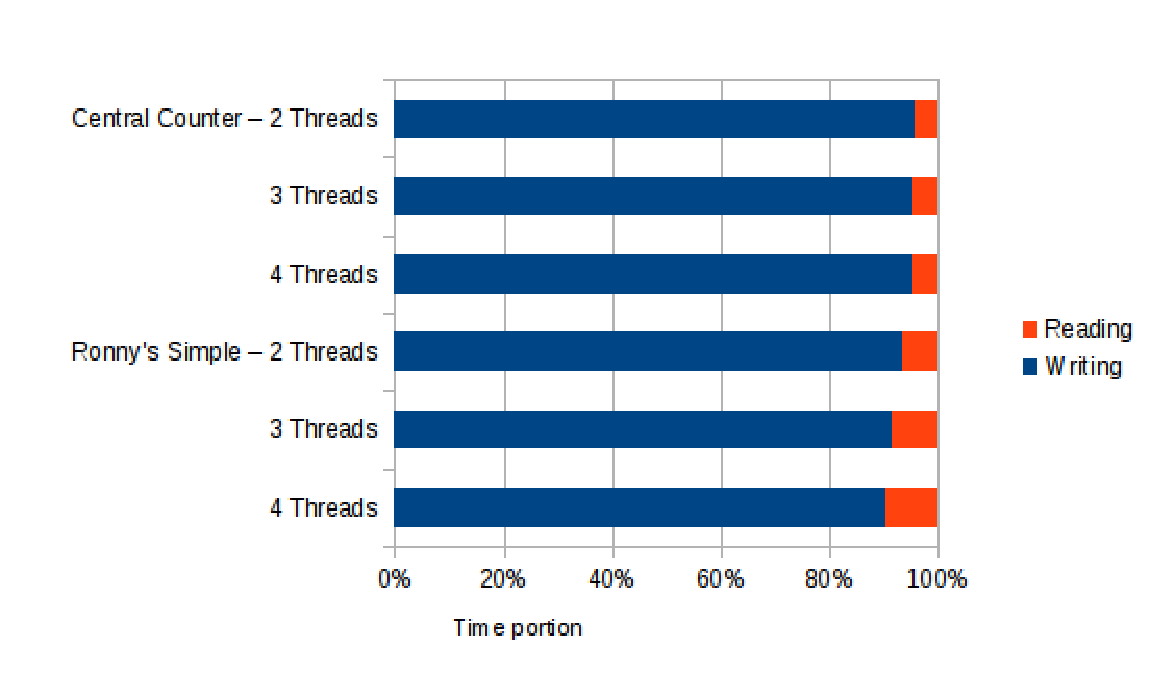
\includegraphics[width=8cm]{charts/cs-work-1000-percent}
						\caption{Percentage of time spent writing vs time spent reading with 1,000 cycles work period}
						\label{fig:cs-work-1000-percent}
					\end{figure}
					\begin{itemize}
						\item less busy waiting due to larger arrival gaps
						\item writing time advantage of ronny's simple is diminished.
						\item ronny's simple reading time increases linearly with the number of threads (2:77, 3:148, 4:218 cycles). Expectation is ~50 across all thread counts in reality.
					\end{itemize}
				\item with larger and more realistic, since 1000 cycles is still very few, work periods this yields a series of writing operations for both algorithms, and a little more time spent reading for ronny's simple barrier.
			\end{itemize}
		\item dissemination vs ronny's fancy
			\begin{itemize}
				\item \todo expected time (last out - last in) (x: threads, y: expected time)
				\item \todo expected time (last out - first out) (x: threads, y: expected time)
				\item number of remote transfers
				\item progress
			\end{itemize}
\label{ssssec:analysis-modelchecking-quantitative-properties-results}

%%%%%%%%%%%%%%%%%%%%%%%%%%%%%%%%%%%%%%%
\subsection{Measurement}
\label{ssec:analysis-measurement}
\begin{itemize}
	\item revisit: http://www.cse.unsw.edu.au/~gernot/benchmarking-crimes.html
	\item don't just give averages. Give at least the standard deviation of benchmarks, too.
	\item give a baseline measurement. Maybe this is possible. The theoretically fastest barrier with instant synchronization. Use the arrival times. Take the maximum. (this should work, shouldn't it?)
	\item central counter vs ronny simple
	\item do not do dissemination vs ronny fancy
	\item ?rapl?
\end{itemize}

%%%%%%%%%%%%%%%%%%%%%%%%%%%%%%%%%%%%%%%
\subsection{Discussion}
\label{ssec:analysis-discussion}
\begin{itemize}
	\item "Discuss and explain your results"
	\item "Show how they support your thesis (or, if they don't, come up with a damned good reason real quick)"
	\item "It is important to separate objective facts clearly from their discussion"
\end{itemize}

%%%%%%%%%%%%%%%%%%%%%%%%%%%%%%%%%%%%%%%%%%%%%%%%%%%%%%%%%%%%%%%%%%%%%%%%%%%%%%%
\section{Conclusion and future work}
\label{sec:conclusion}
conclusion:
\begin{itemize}
	\item "Don't leave it at the discussion: discuss what you/we can learn from the results. Draw some real conclusions. Separate discussion/interpretation of the results clearly from the conclusions you draw from them"
	\item condense results into a small passage
	\item ?repeat claim - overarching thesis - present an answer?
\end{itemize}

Future work:
\begin{itemize}
	\item "Identify all shortcomings/limitations of your work, and discuss how they could be fixed"
	\item evaluate back-off strategies. mwait.
	\item benchmark on Intel system, not only bulldozer. Results might be very different from above benchmarks.
	\item model check more and bigger. Symmetry reduction. Partial order reduction.
		\begin{itemize}
			\item find out at which working period distribution which is better suited. (4 threads in our analysis is nothing)
		\end{itemize}
	\item Make the same comparison again, but with energy consumption.
	\item model multi layered cache. More realistic. Hardware topology
	\item implement ronny fancy on RDMA hardware and benchmark against established algorithms
	\item model ronny fancy and dissemination on shared memory and compare to ronny simple and central counter and reality
	\item explore variations of ronny's barriers
		\begin{itemize}
			\item Ronny's fancy barrier: Try different i increment strategies. Or perhaps randomize the choice of i.
			\item use remote write \& local read instead of local write \& remote read, because remote writing is preferred on some platforms, e.g. on the Epiphany\cite{epiphany}.
		\end{itemize}
\end{itemize}


%%%%%%%%%%%%%%%%%%%%%%%%%%%%%%%%%%%%%%%%%%%%%%%%%%%%%%%%%%%%%%%%%%%%%%%%%%%%%%%
\appendix

%%%%%%%%%%%%%%%%%%%%%%%%%%%%%%%%%%%%%%%%%%%%%%%%%%%%%%%%%%%%%%%%%%%%%%%%%%%%%%%
\pagebreak
\section{Appendix}
\label{sec:appendix}
\subsection{e.g. source code, model source}

%%%%%%%%%%%%%%%%%%%%%%%%%%%%%%%%%%%%%%%%%%%%%%%%%%%%%%%%%%%%%%%%%%%%%%%%%%%%%%%
\pagebreak
\section{Glossary}
\label{sec:glossary}

%%%%%%%%%%%%%%%%%%%%%%%%%%%%%%%%%%%%%%%%%%%%%%%%%%%%%%%%%%%%%%%%%%%%%%%%%%%%%%%
\pagebreak
\section{Bibliography}
\label{sec:bibliography}
\renewcommand\refname{\vskip -1cm} %TODO fine tune perhaps
\nocite{*} % insert not cited references
\bibliographystyle{abbrv}
\bibliography{bibliography}{}

%%%%%%%%%%%%%%%%%%%%%%%%%%%%%%%%%%%%%%%%%%%%%%%%%%%%%%%%%%%%%%%%%%%%%%%%%%%%%%%
\pagebreak
\section{List of Figures}
\label{sec:figures}
\renewcommand{\listfigurename}{\vskip -1cm} %TODO fine tune perhaps
\listoffigures

%%%%%%%%%%%%%%%%%%%%%%%%%%%%%%%%%%%%%%%%%%%%%%%%%%%%%%%%%%%%%%%%%%%%%%%%%%%%%%%
\pagebreak
\section{List of Tables}
\label{sec:tables}
\renewcommand{\listtablename}{\vskip -1cm} %TODO fine tune perhaps
\listoftables

\end{document}
